\documentclass[11pt,a4paper]{article}

% ---------- Page layout & typography ----------
\usepackage[a4paper, top=2.3cm, bottom=2.3cm, left=2.2cm, right=2.2cm, headheight=15pt]{geometry}
\usepackage[T1]{fontenc}
\usepackage[utf8]{inputenc}
\usepackage{lmodern}
\usepackage{microtype}
\usepackage{setspace}
\setstretch{1.06}

% ---------- Math, tables, graphics, lists ----------
\usepackage{amsmath, amssymb}
\usepackage{booktabs}
\usepackage{tabularx}
\usepackage{array}
\usepackage{multirow}
\usepackage{graphicx}
\usepackage{subcaption}
\usepackage{float}
\usepackage{enumitem}
\usepackage{xcolor}
\usepackage{caption}

% ---------- Algorithms ----------
\usepackage{algorithm}
\usepackage{algpseudocode}

% ---------- TikZ diagrams ----------
\usepackage{tikz}
\usetikzlibrary{arrows.meta, positioning, shapes.geometric, calc}

% ---------- Headers & hyperlinks ----------
\usepackage{fancyhdr}
\usepackage[hidelinks, colorlinks=true, linkcolor=navy, citecolor=navy, urlcolor=tealaccent]{hyperref}

% ---------- Color palette (Resonance Navy & Gold) ----------
\definecolor{navy}{RGB}{22, 40, 72}
\definecolor{gold}{RGB}{176, 134, 48}
\definecolor{goldlight}{RGB}{246, 239, 222}
\definecolor{crimson}{RGB}{158, 34, 44}
\definecolor{tealaccent}{RGB}{24, 118, 128}
\definecolor{slate}{RGB}{90, 102, 118}
\definecolor{softblue}{RGB}{234, 240, 248}
\definecolor{softred}{RGB}{252, 236, 238}
\definecolor{softgreen}{RGB}{232, 246, 238}
\definecolor{elhydro}{RGB}{44, 132, 206}
\definecolor{elpyro}{RGB}{212, 76, 46}
\definecolor{elelectro}{RGB}{138, 72, 198}
\definecolor{elanemo}{RGB}{46, 166, 138}
\definecolor{elgeo}{RGB}{192, 146, 42}

\captionsetup{font=small, labelfont=bf, labelsep=colon}
\captionsetup[sub]{font=small, labelfont=bf}
\setlength{\parskip}{3.5pt}
\setlength{\parindent}{0pt}

% Compact Table of Contents spacing so Abstract + full ToC fit cleanly on Page 1
\makeatletter
\renewcommand*\l@section[2]{%
  \ifnum \c@tocdepth >\z@
    \addpenalty\@secpenalty
    \addvspace{0.06em \@plus\p@}%
    \setlength\@tempdima{1.5em}%
    \begingroup
      \parindent \z@ \rightskip \@pnumwidth
      \parfillskip -\@pnumwidth
      \leavevmode \bfseries
      \advance\leftskip\@tempdima
      \hskip -\leftskip
      #1\nobreak\hfil \nobreak\hb@xt@\@pnumwidth{\hss #2}\par
    \endgroup
  \fi}
\renewcommand*\l@subsection{\@dottedtocline{2}{1.5em}{2.3em}}
\makeatother

% Running header/footer for body pages
\pagestyle{fancy}
\fancyhf{}
\fancyhead[L]{\footnotesize\color{slate}\MakeUppercase{Resonance}}
\fancyhead[R]{\footnotesize\color{slate}\MakeUppercase{CSE 3210 -- Final Project Report}}
\fancyfoot[C]{\footnotesize\thepage}
\renewcommand{\headrulewidth}{0.4pt}
\renewcommand{\headrule}{\hbox to\headwidth{\color{gold!60}\leaders\hrule height \headrulewidth\hfill}}

% Compact custom helpers
\newcommand{\fn}[1]{\textsc{#1}}
\newcolumntype{L}[1]{>{\raggedright\arraybackslash}p{#1}}
\newcolumntype{Y}{>{\raggedright\arraybackslash}X}

\begin{document}

% ==============================================================================
% CUSTOM COVER PAGE (Distinct Resonance Executive Design)
% ==============================================================================
\pagenumbering{roman}
\begin{titlepage}
\thispagestyle{empty}
\begin{tikzpicture}[remember picture, overlay]
  % Left architectural accent bar (Navy + Gold pinstripe)
  \fill[navy] (current page.north west) rectangle ([xshift=1.35cm]current page.south west);
  \fill[gold] ([xshift=1.35cm]current page.north west) rectangle ([xshift=1.50cm]current page.south west);
  % Top & bottom delicate gold rule lines on content side
  \draw[gold, line width=1pt] ([xshift=2.3cm, yshift=-1.6cm]current page.north west) -- ([xshift=-1.8cm, yshift=-1.6cm]current page.north east);
  \draw[gold, line width=1pt] ([xshift=2.3cm, yshift=1.8cm]current page.south west) -- ([xshift=-1.8cm, yshift=1.8cm]current page.south east);
\end{tikzpicture}

\hspace*{0.7cm}\begin{minipage}{0.90\textwidth}
\vspace*{0.2cm}

% Institutional Header
{\color{navy}\large\bfseries KHULNA UNIVERSITY OF ENGINEERING \& TECHNOLOGY}\\[0.18cm]
{\color{slate}\normalsize Department of Computer Science and Engineering}

\vspace{1.25cm}

% Custom Vector Resonance Elemental Crest (5 Active Elements + Central Omni Star)
\begin{center}
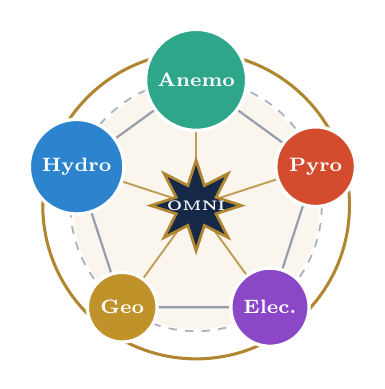
\begin{tikzpicture}[scale=0.95]
  \draw[gold, line width=1.1pt] (0,0) circle (2.05cm);
  \draw[navy!35, dashed, line width=0.7pt] (0,0) circle (1.68cm);
  \fill[goldlight!55] (0,0) circle (1.65cm);

  \draw[navy!45, line width=0.8pt]
    (90:1.68) -- (18:1.68) -- (-54:1.68) -- (-126:1.68) -- (162:1.68) -- cycle;

  \foreach \ang in {90, 18, -54, -126, 162}{
    \draw[gold!80, line width=0.7pt] (0,0) -- (\ang:1.42);
  }

  \node[star, star points=8, star point ratio=2.1, draw=gold, fill=navy,
        line width=1pt, minimum size=1.15cm] (omni) at (0,0) {};
  \node[font=\tiny\bfseries, text=white] at (0,0) {OMNI};

  \node[circle, draw=white, line width=1.2pt, fill=elanemo, minimum size=0.82cm,
        font=\scriptsize\bfseries, text=white] at (90:1.68) {Anemo};
  \node[circle, draw=white, line width=1.2pt, fill=elpyro, minimum size=0.82cm,
        font=\scriptsize\bfseries, text=white] at (18:1.68) {Pyro};
  \node[circle, draw=white, line width=1.2pt, fill=elelectro, minimum size=0.82cm,
        font=\scriptsize\bfseries, text=white] at (-54:1.68) {Elec.};
  \node[circle, draw=white, line width=1.2pt, fill=elgeo, minimum size=0.82cm,
        font=\scriptsize\bfseries, text=white] at (-126:1.68) {Geo};
  \node[circle, draw=white, line width=1.2pt, fill=elhydro, minimum size=0.82cm,
        font=\scriptsize\bfseries, text=white] at (162:1.68) {Hydro};
\end{tikzpicture}
\end{center}

\vspace{0.75cm}

% Title & Subtitle
\begin{center}
  {\color{gold}\scriptsize\bfseries FINAL PROJECT REPORT \;\;$\cdot$\;\;}\\[0.45cm]
  {\color{gold}\scriptsize\bfseries CSE 3210: ARTIFICIAL INTELLIGENCE LABORATORY}\\[0.45cm]
  {\color{navy}\fontsize{30}{34}\selectfont\bfseries RESONANCE}\\[0.25cm]
  
\end{center}

\vspace{1.2cm}

% Clean Framed Metadata Card (Submitted by / Submitted to)
\begin{center}
\fcolorbox{gold!80}{softblue!45}{%
\begin{minipage}{0.92\textwidth}
\vspace{0.35cm}
\begin{tabularx}{\textwidth}{@{}X@{\hspace{1.0cm}}X@{}}
  {\color{crimson}\small\bfseries SUBMITTED BY} &
  {\color{crimson}\small\bfseries SUBMITTED TO} \\[0.22cm]
  \textbf{Md.\ Sadikul Islam Siyam} &
  \textbf{Waliul Islam Sumon} \\
  {\small Roll: 2207031} &
  {\small Lecturer, Department of CSE, KUET} \\[0.32cm]
  \textbf{Rupam Bose} &
  \textbf{Mst.\ Sadia Islam} \\
  {\small Roll: 2207038} &
  {\small Lecturer, Department of CSE, KUET} \\
\end{tabularx}
\vspace{0.35cm}
\end{minipage}}
\end{center}

\vfill

\begin{center}
  {\small\color{slate}\textbf{Date of Submission:} 23 November 2026}
\end{center}
\vspace{0.4cm}
\end{minipage}
\end{titlepage}

% ==============================================================================
% PAGE 1: ABSTRACT + TABLE OF CONTENTS
% ==============================================================================
\pagenumbering{arabic}
\setcounter{page}{1}

\begin{center}
  {\large\bfseries\color{navy} Abstract}
\end{center}
\vspace{-0.25cm}
\begin{quote}\small
\textbf{Resonance} is a two-player, turn-based tactical collectible card game built in \textbf{Godot~4} and themed around the \emph{Avatar} universe. Each player commands three characters and a 20-card action deck, spending a stochastic pool of eight elemental dice per round to cast attacks, trigger elemental reactions, equip signature weapons, and chain fast utility cards. To handle hidden hands, random dice, and asymmetric Fast-versus-Combat turns, our engine integrates six AI techniques across three difficulty tiers (\emph{Easy}, \emph{Normal}, \emph{Hard}): a Sugeno Fuzzy Logic profiler, an informed A* Lethal Planner, Iterative-Deepening Alpha-Beta Minimax with zero-cost fast-action depth handling, Shortlisted Information-Set Monte Carlo Tree Search (IS-MCTS), and a Minimum Remaining Values (MRV) Forward-Checking CSP solver for smart dice payment and deck auto-completion. This report presents the game overview, rules and mechanics, formal game model, system design, all AI algorithms with domain modifications, an engine-verified step-by-step decision tree analysis, and a 12-game tournament benchmark.
\end{quote}

\vspace{-0.35cm}
{\footnotesize\setstretch{0.89}\tableofcontents}
\newpage

% ==============================================================================
% SECTION 1: INTRODUCTION
% ==============================================================================
\section{Introduction}

In classical turn-based games such as Chess or WordBattle, every state transition is deterministic and both players observe the entire board. In a tactical collectible card game (TCG), however, every move simultaneously manages multiple coupled uncertainties: the opponent holds hidden cards in hand, both players draw from shuffled decks, every round begins with a random pool of elemental dice, and a single turn may chain several \emph{fast} preparation cards before ending with a \emph{combat} attack or character switch. Choosing a move that deals high immediate damage can leave a character exposed to a devastating elemental reaction on the opponent's very next reply.

\textbf{Resonance: Genius Invokation TCG (Avatar Edition)} was developed to study how multiple classical and modern Artificial Intelligence techniques cooperate inside a single, complete, playable tabletop game. Rather than relying on one monolithic heuristic, our engine combines six complementary AI paradigms—\emph{Fuzzy Logic}, \emph{A* Search}, \emph{Alpha-Beta Minimax}, \emph{Information-Set MCTS}, \emph{Imperfect-Information Determinization}, and \emph{Constraint Satisfaction}—backed by a deterministic, data-driven rules engine in Godot~4.

% ==============================================================================
% SECTION 2: GAME OVERVIEW
% ==============================================================================
\section{Game Overview}

\textbf{Resonance} pits two players against each other on an ornate tabletop arena. Each player enters a match with \textbf{3 distinct character cards} (10~HP and 1~Max Energy each) and a \textbf{20-card action deck} (at most 2 copies of any card). A match runs across a sequence of rounds until all three characters on one side are defeated. Every player slot can be controlled by a human or by the AI across three selectable difficulty tiers, supporting \emph{Human vs.\ AI}, \emph{Human vs.\ Human (same device with hotseat privacy cover)}, and \emph{AI vs.\ AI (spectate)} modes. Table~\ref{tab:match-settings} summarizes the core match parameters.

\begin{table}[H]
\centering
\caption{Core match settings and deck rules in Resonance.}
\label{tab:match-settings}
\small
\begin{tabularx}{\textwidth}{@{}L{2.7cm} Y L{3.1cm}@{}}
\toprule
Setting & Options / Rule & Default \\
\midrule
Match Mode & Human vs.\ AI, Human vs.\ Human, AI vs.\ AI & Human vs.\ AI \\
AI Difficulty & Easy (Fuzzy 1-ply), Normal (A* + Alpha-Beta), Hard (A* + AB + IS-MCTS) & Normal \\
Team & 3 distinct characters from 6-character roster & Preset or Custom \\
Action Deck & Exactly 20 cards, max 2 copies per card, character-legal & Preset / CSP Auto-fill \\
Preset Decks & \emph{Team Avatar}, \emph{Fire Nation Royals}, \emph{Lotus \& Rebels} & Any selectable \\
Opening Hand & Draw 5 cards at start (1 mulligan); max hand 10; draw 2 per End Phase & 5 start / 2 end \\
Elemental Dice & 8 dice rolled per round (1 free reroll); max pool 16 via Carryover & 8 per round \\
\bottomrule
\end{tabularx}
\end{table}

\subsection{Rounds and Phase Flow}

Every match begins with a coin toss determining the Round~1 starting player, followed by a \textbf{Setup Phase} (card mulligan and starting active character selection). Once Setup finishes, gameplay loops through repeating \textbf{Rounds}, each structured into three phases:
\begin{enumerate}[leftmargin=1.4em, itemsep=2pt]
  \item \textbf{Roll Phase:} Both players roll 8 elemental dice (plus any carried-over Omni dice from the previous round, up to 16 total) and receive \textbf{1 free reroll} to re-throw any unwanted dice before locking their pool.
  \item \textbf{Action Phase:} Starting with the player who holds initiative, players alternate turns spending dice to cast character skills, play equipment or utility cards, switch their active character, tune dice, or declare \emph{End Round}. The first player to declare \emph{End Round} secures first-player initiative for the next round.
  \item \textbf{End Phase:} Once both players have declared \emph{End Round}, end-of-round statuses expire (clearing \emph{Stunned}, \emph{Attack +1}, etc.), any active \emph{Dice Carryover} stores remaining dice as Omni dice for the next round, both players draw 2 cards, and the next round begins.
\end{enumerate}

\subsection{Elements and the 8-Dice Economy}

The engine defines six elemental identities (\emph{Hydro}, \emph{Pyro}, \emph{Electro}, \emph{Anemo}, \emph{Geo}, and \emph{Cryo}), alongside \emph{Omni} (universal wildcard), \emph{Physical} (non-elemental damage), and \emph{Piercing} (unblockable bypass damage). Because the finalized six-character Avatar roster spans the five bending/combat elements—\textbf{Hydro, Pyro, Electro, Anemo, and Geo}—\textbf{Cryo is excluded from dice rolls} so players never roll dead dice. Each rolled die draws independently from a 6-face weighted distribution:
\begin{equation}
  P(\text{Omni}) = \frac{1}{8} = 12.5\%, \qquad
  P(e) = \frac{7}{40} = 17.5\% \quad \forall\, e \in \{\text{Hydro}, \text{Pyro}, \text{Electro}, \text{Anemo}, \text{Geo}\}.
\end{equation}

Every skill and action card specifies one of three dice-cost patterns:
\begin{itemize}[leftmargin=1.4em, itemsep=2pt]
  \item \textbf{Aligned (Exact) Cost:} Requires $n$ dice matching a specific element (or Omni) plus $u$ \emph{unaligned} dice of any face (e.g., Aang's \emph{Air Gust} costs 2~Anemo + 1~Any).
  \item \textbf{Unaligned (Any) Cost:} Paid using any combination of dice faces (e.g., switching active character costs 1~Any; \emph{Draw Cards} costs 1~Any).
  \item \textbf{Same-Type Cost:} Used by signature weapons (2~Same-Type dice)—requires 2 dice sharing \emph{any} identical element, with Omni acting as a wild match.
\end{itemize}
Whenever dice rolls miss the active character's element, players can perform \textbf{Elemental Tuning}: discarding any card from hand to convert one non-matching, non-Omni die into the active character's element as a fast action.

\subsection{Elemental Reactions}

Dealing \textbf{Hydro}, \textbf{Pyro}, or \textbf{Electro} damage (or \emph{Cryo} in general engine rules) attaches that element as a persistent \textbf{aura} on the target. Striking an aura-affected character with a reactive second element consumes the aura and triggers an \textbf{Elemental Reaction}. \textbf{Anemo} and \textbf{Geo} never leave an aura themselves; instead, they react immediately against any existing aura. Table~\ref{tab:reactions} lists every active reaction in Resonance. (The underlying rules engine also preserves Cryo reactions—\emph{Melt}~$+2$, \emph{Superconduct}~$+1$ + 1~Piercing, and \emph{Frozen}~$+1$ + freeze—for future roster expansion.)

\begin{table}[H]
\centering
\caption{Active elemental reactions in Resonance (Avatar roster).}
\label{tab:reactions}
\small
\begin{tabularx}{\textwidth}{@{}L{2.4cm} L{2.25cm} c L{4.55cm} Y@{}}
\toprule
Reaction & Elements & Bonus & Secondary Effect & Tactical Role \\
\midrule
\textbf{Vaporize} & Hydro + Pyro & $+1$ & None & Efficient burst damage amplification. \\
\textbf{Overloaded} & Pyro + Electro & $+2$ & Force-switch target to next living ally & High burst plus board disruption; breaks enemy setups. \\
\textbf{Electro-Charged} & Hydro + Electro & $+1$ & 1~Piercing DMG to all standby foes & Chips the entire opposing bench through shields. \\
\textbf{Swirl} & Anemo + Aura & $+0$ & \textbf{Aang:} 2 swirled Elemental DMG to standby foes (1 generic) & Spreads aura and heavy AoE damage across enemy bench. \\
\textbf{Crystallize} & Geo + Aura & $+1$ & Attacker gains \emph{Crystallize Shield} (+1, max 2) & Converts enemy aura into defensive tempo. \\
\bottomrule
\end{tabularx}
\end{table}

\subsection{Character Roster and Action Cards}

Every character begins with \textbf{10~HP} and \textbf{1~Max Energy}, ensuring fast-paced Elemental Bursts that reward smart energy timing. Normal Attacks and Elemental Skills each grant $+1$~Energy; Elemental Bursts spend 1~Energy for a high-impact signature move. Table~\ref{tab:characters} lists all six characters, and Table~\ref{tab:cards} catalogs all 15 action cards.

\begin{table}[H]
\centering
\caption{All six playable Avatar characters (each has 10~HP and 1~Max Energy). Costs list Aligned + Any dice.}
\label{tab:characters}
\small
\begin{tabularx}{\textwidth}{@{}L{1.45cm} L{1.2cm} L{2.95cm} L{2.75cm} Y@{}}
\toprule
Character & Elem. & Normal (1+2) & Skill (2+1) & Burst / Ultimate (3 Elem.\ + 1 Energy) \\
\midrule
\textbf{Aang} & Anemo & \emph{Air Jab}: 2~Phys & \emph{Air Gust}: 2~Anemo & \emph{Avatar Cleansing}: 4~Anemo + cleanse own aura (\emph{Passive}: Swirls deal \textbf{2}~DMG to standby foes) \\
\textbf{Zuko} & Pyro & \emph{Flame Slash}: 2~Phys & \emph{Fire Whip}: 3~Pyro & \emph{Dragon's Roar}: 3~Pyro + 1~Piercing to standby foes \\
\textbf{Katara} & Hydro & \emph{Water Whip}: 1~Phys & \emph{Tidal Wave}: 2~Hydro & \emph{Healing Waters}: 3~Hydro + heal all living allies 1~HP (+2 extra with \emph{Spirit Water}) \\
\textbf{Azula} & Electro & \emph{Lightning Strike}: 2~Phys & \emph{Blue Arc}: 2~Electro & \emph{Thunder Judgement}: 3~Electro + apply \emph{Stunned} to struck target (even after Overloaded switch) \\
\textbf{Toph} & Geo & \emph{Rock Smash}: 2~Phys & \emph{Earth Pillar}: 3~Geo & \emph{Metal Fortress}: 3~Geo + team combat status \emph{Shield +2} \\
\textbf{Iroh} & Pyro & \emph{Tea Master Strike}: 2~Phys & \emph{Breath of Fire}: 3~Pyro & \emph{Dragon of the West}: 4~Pyro + team \emph{Attack +1} for the round \\
\bottomrule
\end{tabularx}
\end{table}

\begin{table}[H]
\centering
\caption{All 15 action cards: 6 character-specific Equipment cards and 9 shared Utility event cards.}
\label{tab:cards}
\small
\begin{tabularx}{\textwidth}{@{}L{1.65cm} L{4.65cm} L{1.25cm} Y@{}}
\toprule
Category & Card Name & Cost & Effect \\
\midrule
\multirow{6}{*}{Equipment}
 & \emph{Aang's Glider Staff} & 2 Same & Equip to Aang: attacks deal $+1$~DMG. \\
 & \emph{Zuko's Dual Broadswords} & 2 Same & Equip to Zuko: attacks deal $+1$~DMG. \\
 & \emph{Azula's Dagger} & 2 Same & Equip to Azula: attacks deal $+1$~DMG. \\
 & \emph{Earth Rumble Championship Belt} & 2 Same & Equip to Toph: attacks deal $+1$~DMG. \\
 & \emph{Iroh's Pearl-Handled Dagger} & 2 Same & Equip to Iroh: attacks deal $+1$~DMG. \\
 & \emph{Katara's Spirit Water} & 1 Any & Equip to Katara: Katara's Ultimate heals $+2$ extra HP per ally. \\
\midrule
\multirow{9}{*}{Utility}
 & \emph{Reroll Dice} & 0 & Automatically reroll all non-matching, non-Omni dice. \\
 & \emph{Swap Cards} & 0 & Return up to 2 chosen hand cards to deck after drawing replacements. \\
 & \emph{Elemental Dice} & 0 & Gain 1 die matching active character's element. \\
 & \emph{Active Character Healing}$^\dagger$ & 0 & Heal active character for 1~HP. \\
 & \emph{Draw Cards} & 1 Any & Draw 2 cards from deck. \\
 & \emph{Dice Carryover} & 1 Any & Unused dice at End Phase carry into next round as Omni dice. \\
 & \emph{Omni Conversion} & 1 Any & Convert up to 3 off-element dice into Omni dice. \\
 & \emph{Dual Character Healing}$^\dagger$ & 1 Any & Heal active character and lowest-HP living standby ally for 1~HP each. \\
 & \emph{Party Healing}$^\dagger$ & 2 Any & Heal every living party member for 1~HP. \\
\bottomrule
\multicolumn{4}{@{}l@{}}{\footnotesize $^\dagger$Healing action cards share a once-per-round limit per player.}
\end{tabularx}
\end{table}

% ==============================================================================
% SECTION 3: RULES AND MECHANICS
% ==============================================================================
\section{Rules and Mechanics}

\subsection{Match Rules in Plain Language}

\begin{enumerate}[leftmargin=1.4em, itemsep=2.5pt]
  \item \textbf{Deck Legality:} A legal deck has exactly 3 distinct characters and 20 action cards, with at most 2 copies of any card. Character equipment cards may only be included if that character is on the 3-character team.
  \item \textbf{Setup and Mulligan:} Both players shuffle their decks and draw 5 cards. Starting with the coin-toss winner, each player may select any number of cards to replace once (\emph{Mulligan}); replacements are drawn \emph{before} returned cards are shuffled back so a player never redraws the exact discarded card. Each player then selects their starting \emph{Active Character}.
  \item \textbf{Roll Phase:} At the start of every round, each player rolls 8 dice (plus any Omni dice carried over from \emph{Dice Carryover}, capped at 16). Each player gets one free reroll of any subset of dice, then confirms their dice pool to start the Action Phase.
  \item \textbf{Fast Actions vs.\ Combat Actions:} The Action Phase distinguishes two action speeds (Table~\ref{tab:fast-combat}). You may chain as many \emph{Fast Actions} as you can afford on a single turn without giving up control. The moment you execute a \emph{Combat Action}, your turn immediately passes to the opponent (unless the opponent has already ended the round, in which case you keep acting until you also declare \emph{End Round}).
  \item \textbf{Energy and Elemental Bursts:} Using a Normal Attack or Elemental Skill grants $+1$~Energy (capped at 1). When at full energy (1/1), the active character may pay 3 aligned dice plus 1~Energy to cast their Elemental Burst.
  \item \textbf{Healing Rules:} To prevent stalling, each player may play \textbf{at most one healing action card} (\emph{Active}, \emph{Dual}, or \emph{Party Healing}) per round; the flag resets at the start of the next round. \emph{Dual Character Healing} specifically heals the active character plus the \emph{lowest-HP injured living standby} character (never double-healing the active unit). Katara's \emph{Healing Waters} Burst is a character skill rather than an action card, so it is unaffected by the card cap, and \emph{Katara's Spirit Water} boosts only her Ultimate healing ($1 \to 3$~HP per living ally).
  \item \textbf{Crowd Control (\emph{Stunned}) and Cleansing:} A \emph{Stunned} character cannot use skills until End Phase, though the player can still play cards, tune dice, or switch out. When Azula's \emph{Thunder Judgement} strikes a Pyro-affected target, \emph{Overloaded} forces the target to switch out—our engine records the struck target before the switch so \emph{Stunned} lands on the character who actually took the hit, not the incoming replacement. Conversely, Aang's \emph{Avatar Cleansing} removes any elemental aura attached to Aang himself, preventing incoming reactions.
  \item \textbf{Knockouts and Victory:} When a character's HP drops to 0, they are defeated (losing aura, statuses, energy, and equipment). If the active character is defeated and living allies remain, that player must immediately choose a replacement active character. The first player to defeat all 3 opposing characters wins immediately.
\end{enumerate}

\begin{table}[H]
\centering
\caption{Fast Actions versus Combat Actions during the Action Phase.}
\label{tab:fast-combat}
\small
\begin{tabularx}{\textwidth}{@{}L{2.35cm} L{7.4cm} Y@{}}
\toprule
Action Speed & Actions Included & Turn-Passing Behavior \\
\midrule
\textbf{Fast Action} & Play Equipment card, play Utility Event card, Elemental Tuning (discard 1 card to convert 1 die to active element) & \textbf{Keeps turn:} the same player immediately acts again. \\
\textbf{Combat Action} & Cast Normal Attack / Skill / Burst, manual Switch (1~Any die), declare \emph{End Round} & \textbf{Passes turn} to opponent (unless opponent already ended the round). \\
\bottomrule
\end{tabularx}
\end{table}

\subsection{The Six-Step Damage and Reaction Pipeline}

Every attack passes through a strict, deterministic six-stage pipeline inside \texttt{TCGRulesEngine.deal\_damage}, illustrated in Figure~\ref{fig:damage-pipeline}. Because both the UI damage-forecast preview and all AI simulations call this exact same pipeline, previewed numbers and AI look-ahead predictions never disagree with live combat.

\begin{figure}[H]
\centering
\resizebox{\textwidth}{!}{%
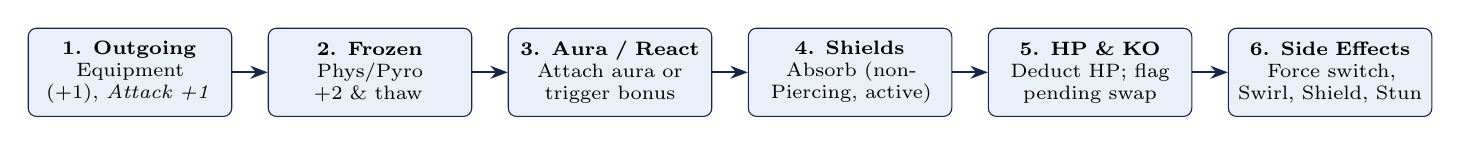
\begin{tikzpicture}[
  node distance=0.45cm,
  stepbox/.style={rectangle, rounded corners=3pt, draw=navy, fill=softblue,
                  minimum height=1.12cm, text width=2.35cm, align=center, font=\scriptsize},
  arr/.style={-{Stealth[length=2.2mm]}, thick, color=navy}
]
  \node[stepbox] (s1) {\textbf{1. Outgoing}\\Equipment ($+1$), \emph{Attack +1}};
  \node[stepbox, right=of s1] (s2) {\textbf{2. Frozen}\\Phys/Pyro $+2$ \& thaw};
  \node[stepbox, right=of s2] (s3) {\textbf{3. Aura / React}\\Attach aura or trigger bonus};
  \node[stepbox, right=of s3] (s4) {\textbf{4. Shields}\\Absorb (non-Piercing, active)};
  \node[stepbox, right=of s4] (s5) {\textbf{5. HP \& KO}\\Deduct HP; flag pending swap};
  \node[stepbox, right=of s5] (s6) {\textbf{6. Side Effects}\\Force switch, Swirl, Shield, Stun};
  \draw[arr] (s1) -- (s2);
  \draw[arr] (s2) -- (s3);
  \draw[arr] (s3) -- (s4);
  \draw[arr] (s4) -- (s5);
  \draw[arr] (s5) -- (s6);
\end{tikzpicture}}
\caption{The deterministic six-step damage and reaction pipeline executed for every strike.}
\label{fig:damage-pipeline}
\end{figure}

\subsection{Worked Combat Example}

Suppose it is Round~2, Action Phase. Player~1's active \textbf{Aang} (6~HP, 1/1~Energy, \textbf{Pyro} aura) faces Player~2's active \textbf{Azula} (5~HP, 1/1~Energy, \textbf{Hydro} aura), with \textbf{Zuko} (6~HP) and \textbf{Iroh} (8~HP) on Player~2's bench. Player~1 holds \emph{Active Character Healing} and 4 dice (\texttt{Anemo, Anemo, Omni, Pyro}).
\begin{enumerate}[leftmargin=1.4em, itemsep=2pt]
  \item Player~1 first plays \textbf{Active Character Healing} (0 dice, \emph{Fast Action}): Aang heals $6 \to 7$~HP, the once-per-round healing flag activates, and Player~1 \textbf{keeps the turn}.
  \item Player~1 next casts \textbf{Avatar Cleansing} (3~Anemo paid via \texttt{Anemo, Anemo, Omni} + 1~Energy, \emph{Combat Action}):
  \begin{itemize}[leftmargin=1.3em, itemsep=1pt]
    \item \emph{Step 3--5:} Base 4~Anemo DMG hits Hydro-affected Azula, consuming her Hydro aura and triggering \textbf{Swirl (Hydro)}. Azula drops $5 \to 1$~HP.
    \item \emph{Step 6 (Aang's Passive Swirl):} Because Aang is the caster, Swirl deals \textbf{2~Hydro DMG} (rather than 1) to both standby foes: Zuko drops $6 \to 4$~HP and Iroh drops $8 \to 6$~HP, and both receive a \textbf{Hydro aura}.
    \item \emph{Skill Step 2 (Self-Cleanse):} Aang clears his own Pyro aura, then the turn passes to Player~2.
  \end{itemize}
  \item Now Player~2 replies with Azula's \textbf{Thunder Judgement} (3~Electro + 1~Energy). Because Aang cleansed his Pyro aura, \textbf{no Overloaded reaction occurs}: Azula deals only 3~Electro DMG ($7 \to 4$~HP), attaches Electro aura, and stuns Aang—avoiding the lethal $+2$ Overloaded bonus and forced switch that would have happened without cleansing.
\end{enumerate}

% ==============================================================================
% SECTION 4: GAME MODEL
% ==============================================================================
\section{Game Model}

To apply formal AI search and planning algorithms, we represent Resonance as an adversarial state-transition game.

\textbf{State.} A complete game state is the 8-tuple
\begin{equation}
  s = \langle P_0, P_1, \text{phase}, r, \text{cur}, \text{first}, \text{ender}, \text{pending} \rangle,
\end{equation}
where $\text{phase} \in \{\text{setup}, \text{roll}, \text{action}, \text{end}, \text{over}\}$, $r \ge 1$ is the round counter, $\text{cur} \in \{0,1\}$ is the active actor in the Action Phase, $\text{first} \in \{0,1\}$ holds round initiative, $\text{ender} \in \{-1,0,1\}$ records who ended the round first ($-1$ if neither), and $\text{pending}$ is a queue of players who must immediately replace a defeated active character. Each player record is
\begin{equation}
  P_i = \langle C_i, a_i, D_i, H_i, K_i, B_i, e_i, h_i \rangle,
\end{equation}
containing the three character instances $C_i$ (each storing HP, energy, aura, equipment, statuses, and defeat flag), active index $a_i \in \{-1,0,1,2\}$, dice pool $D_i$, hand $H_i$, remaining deck $K_i$, team combat statuses $B_i$, round-ended flag $e_i$, and healing-card-used flag $h_i$.

\textbf{The Six Formal Search Functions.}
\begin{itemize}[leftmargin=1.4em, itemsep=2pt]
  \item \textbf{$S_0$ (Initial State):} Both teams start with 3 characters at 10~HP and 0~Energy, shuffled 20-card decks, 5 drawn cards, $\text{phase} = \text{setup}$, $r = 1$, and $\text{first} \in \{0,1\}$ set by coin toss.
  \item \textbf{\fn{Player}($s$):} Returns the player who must act next: the head of $\text{pending}$ if non-empty; otherwise the next unfinished player in Setup or Roll order; otherwise $\text{cur}$ during Action Phase; or $-1$ when $\text{phase} = \text{over}$.
  \item \textbf{\fn{Actions}($s$):} Returns all legal atomic actions for $\fn{Player}(s)$: \texttt{mulligan} / \texttt{choose\_active} in Setup; \texttt{reroll} / \texttt{confirm\_roll} in Roll; and affordable \texttt{skill}, \texttt{switch}, \texttt{card}, \texttt{tune}, and \texttt{end\_round} actions in Action Phase (typically 5--18 actions after de-duplicating identical card copies and tuning faces).
  \item \textbf{\fn{Result}($s, a$):} Validates dice payment and legality, deducts dice/cards/energy, executes the 6-step damage pipeline or card effect, checks knockouts and victory, and updates $\text{cur}$ (retaining control for Fast Actions, passing control for Combat Actions).
  \item \textbf{\fn{Terminal}($s$):} True iff all three characters of $P_0$ or $P_1$ (or both) are defeated ($\text{phase} = \text{over}$).
  \item \textbf{\fn{Utility}($s$):} Zero-sum terminal payoff for player $i$: $+6.0$ for a win, $0.0$ for a draw, and $-6.0$ for a loss in Alpha-Beta (mapped to $1.0 / 0.5 / 0.0$ in IS-MCTS).
\end{itemize}

Figures~\ref{fig:model-turn} and~\ref{fig:model-result} illustrate \fn{Player}($s$), \fn{Actions}($s$), \fn{Result}($s,a$), and \fn{Terminal}($s$) on concrete Avatar game states.

\begin{figure}[H]
\centering
\resizebox{\textwidth}{!}{%
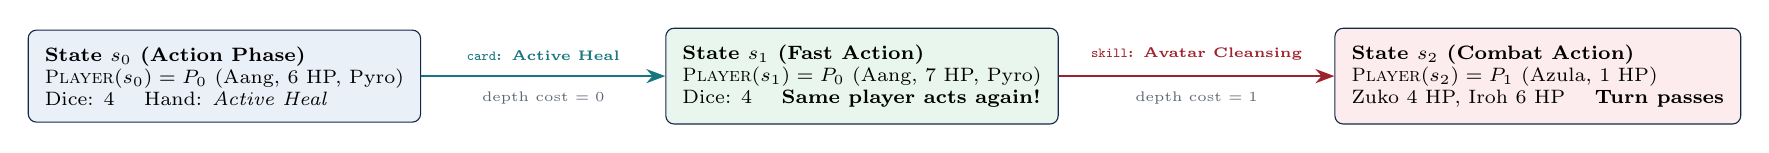
\begin{tikzpicture}[
  box/.style={rectangle, rounded corners=3pt, draw=navy, fill=softblue, inner sep=6pt, font=\scriptsize, align=left},
  fast/.style={-{Stealth[length=2.4mm]}, thick, color=tealaccent},
  comb/.style={-{Stealth[length=2.4mm]}, thick, color=crimson}
]
  \node[box] (s0) {\textbf{State $s_0$ (Action Phase)}\\
    $\fn{Player}(s_0) = P_0$ (Aang, 6~HP, Pyro)\\
    Dice: 4 \quad Hand: \emph{Active Heal}};
  \node[box, right=3.1cm of s0, fill=softgreen] (s1) {\textbf{State $s_1$ (Fast Action)}\\
    $\fn{Player}(s_1) = P_0$ (Aang, 7~HP, Pyro)\\
    Dice: 4 \quad \textbf{Same player acts again!}};
  \node[box, right=3.5cm of s1, fill=softred] (s2) {\textbf{State $s_2$ (Combat Action)}\\
    $\fn{Player}(s_2) = P_1$ (Azula, 1~HP)\\
    Zuko 4~HP, Iroh 6~HP \quad \textbf{Turn passes}};
  \draw[fast] (s0) -- node[above=2pt, font=\tiny\bfseries, color=tealaccent] {\texttt{card}: Active Heal} node[below=2pt, font=\tiny, color=slate] {depth cost $= 0$} (s1);
  \draw[comb] (s1) -- node[above=2pt, font=\tiny\bfseries, color=crimson] {\texttt{skill}: Avatar Cleansing} node[below=2pt, font=\tiny, color=slate] {depth cost $= 1$} (s2);
\end{tikzpicture}}
\caption{\fn{Player}($s$) and asymmetric turn transitions: Fast Actions retain control ($P_0 \to P_0$) while Combat Actions pass control ($P_0 \to P_1$).}
\label{fig:model-turn}
\end{figure}

\begin{figure}[H]
\centering
\resizebox{0.92\textwidth}{!}{%
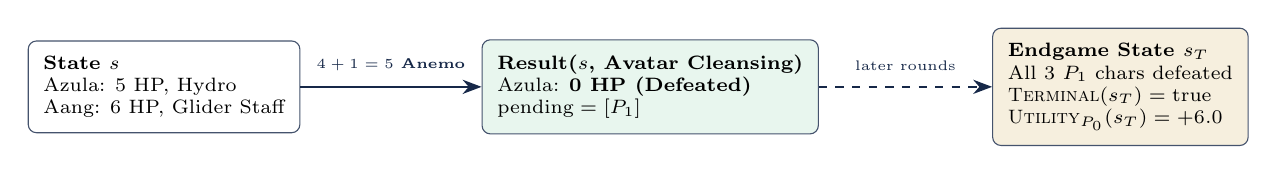
\begin{tikzpicture}[
  st/.style={rectangle, rounded corners=3pt, draw=navy!80, fill=white, inner sep=5.5pt, font=\scriptsize, align=left},
  arr/.style={-{Stealth[length=2.4mm]}, thick, color=navy}
]
  \node[st] (r0) {\textbf{State $s$}\\Azula: 5~HP, Hydro\\Aang: 6~HP, Glider Staff};
  \node[st, right=2.3cm of r0, fill=softgreen] (r1) {\textbf{\fn{Result}($s$, Avatar Cleansing)}\\Azula: \textbf{0~HP (Defeated)}\\$\text{pending} = [P_1]$};
  \node[st, right=2.2cm of r1, fill=goldlight] (r2) {\textbf{Endgame State $s_T$}\\All 3 $P_1$ chars defeated\\$\fn{Terminal}(s_T) = \text{true}$\\$\fn{Utility}_{P_0}(s_T) = +6.0$};
  \draw[arr] (r0) -- node[above=2pt, font=\tiny\bfseries] {$4+1=5$ Anemo} (r1);
  \draw[arr, dashed] (r1) -- node[above=2pt, font=\tiny] {later rounds} (r2);
\end{tikzpicture}}
\caption{\fn{Result}($s,a$), knockout handling, \fn{Terminal}($s$), and \fn{Utility}($s$).}
\label{fig:model-result}
\end{figure}

\textbf{Classification of the Game.} Unlike deterministic, fully observable board games, Resonance is:
\begin{enumerate}[leftmargin=1.4em, itemsep=1pt]
  \item \textbf{Two-player and zero-sum:} Every HP gain, knockout, or tempo advantage for $P_0$ directly diminishes $P_1$'s winning chances ($\text{Eval}(s, 0) = -\text{Eval}(s, 1)$).
  \item \textbf{Stochastic:} Dice rolls, rerolls, and deck shuffles introduce random chance events across rounds.
  \item \textbf{Partially observable (imperfect information):} Players observe both teams, HP, energy, auras, dice counts, and public plays, but cannot see the opponent's hand or either deck order.
  \item \textbf{Asymmetric multi-action per turn:} Fast actions keep the turn while combat actions pass it, creating horizon artifacts if search depth counts all actions equally.
\end{enumerate}
Because of these four properties, plain textbook Minimax is insufficient on its own—motivating our hybrid architecture combining determinization, Fuzzy evaluation, A* lethal planning, zero-cost-fast Alpha-Beta, IS-MCTS, and CSP dice solving.

% ==============================================================================
% SECTION 5: SYSTEM DESIGN
% ==============================================================================
\section{System Design}

Resonance is implemented in \textbf{Godot~4.7.2 (GDScript)} using a strict separation between presentation, authoritative rules simulation, declarative JSON content, and AI search. Figure~\ref{fig:architecture} illustrates the five architectural layers.

\begin{figure}[H]
\centering
\resizebox{0.96\textwidth}{!}{%
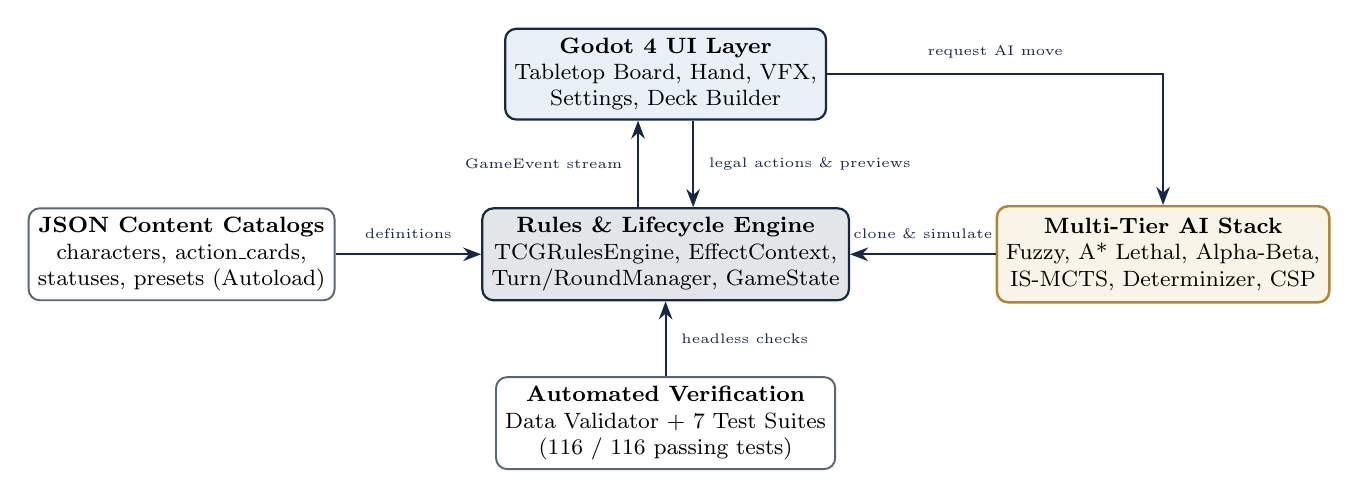
\begin{tikzpicture}[
  box/.style={rectangle, rounded corners=4pt, draw=navy, line width=0.8pt, fill=softblue,
              minimum width=3.9cm, minimum height=1.15cm, align=center, font=\footnotesize},
  side/.style={rectangle, rounded corners=4pt, draw=slate, line width=0.7pt, fill=white,
               minimum width=3.5cm, minimum height=1.15cm, align=center, font=\footnotesize},
  ai/.style={rectangle, rounded corners=4pt, draw=gold, line width=0.9pt, fill=goldlight!70,
             minimum width=3.9cm, minimum height=1.22cm, align=center, font=\footnotesize},
  arr/.style={-{Stealth[length=2.3mm]}, thick, color=navy}
]
  \node[box] (ui) {\textbf{Godot 4 UI Layer}\\Tabletop Board, Hand, VFX,\\Settings, Deck Builder};
  \node[box, below=1.1cm of ui, fill=navy!12] (engine) {\textbf{Rules \& Lifecycle Engine}\\TCGRulesEngine, EffectContext,\\Turn/RoundManager, GameState};
  \node[side, left=1.85cm of engine] (data) {\textbf{JSON Content Catalogs}\\characters, action\_cards,\\statuses, presets (Autoload)};
  \node[ai, right=1.85cm of engine] (ai) {\textbf{Multi-Tier AI Stack}\\Fuzzy, A* Lethal, Alpha-Beta,\\IS-MCTS, Determinizer, CSP};
  \node[side, below=0.95cm of engine] (tests) {\textbf{Automated Verification}\\Data Validator + 7 Test Suites\\(116 / 116 passing tests)};

  \draw[arr] ([xshift=0.35cm]ui.south) -- node[right=2pt, font=\tiny] {legal actions \& previews} ([xshift=0.35cm]engine.north);
  \draw[arr] ([xshift=-0.35cm]engine.north) -- node[left=2pt, font=\tiny] {GameEvent stream} ([xshift=-0.35cm]ui.south);
  \draw[arr] (data) -- node[above=2pt, font=\tiny] {definitions} (engine);
  \draw[arr] (ai) -- node[above=2pt, font=\tiny] {clone \& simulate} (engine);
  \draw[arr] (ui.east) -| node[pos=0.25, above=2pt, font=\tiny] {request AI move} (ai.north);
  \draw[arr] (tests) -- node[right=2pt, font=\tiny] {headless checks} (engine);
\end{tikzpicture}}
\caption{Modular software architecture of Resonance in Godot~4. The UI previews and AI simulations both invoke the exact same deterministic \texttt{TCGRulesEngine}.}
\label{fig:architecture}
\end{figure}

Crucially, \texttt{TCGGameState.clone(keep\_log=false, share\_rng=true)} disables UI event logging (\texttt{track\_events = false}) during AI search, producing lightweight state snapshots so Alpha-Beta and IS-MCTS can simulate thousands of positions cleanly without ever mutating the live match state or triggering visual animations.

\subsection{Data-Driven Catalogs and Deck Validation}

All 6 characters, 15 action cards, 11 statuses, and 3 preset decks live in external JSON files under \texttt{GodotTCG/data/} loaded by the \texttt{CardDataSystem} autoload singleton. Skills and action cards compile into declarative opcode sequences (\texttt{damage}, \texttt{piercing\_others}, \texttt{heal\_dual}, \texttt{clear\_self\_aura}, \texttt{foe\_char\_status}, \texttt{convert\_to\_omni}, etc.) executed by \texttt{TCGEffectContext}. Decks can be auto-completed by the CSP solver, persisted locally via \texttt{TCGDeckStore}, and exported or imported using compact URL-safe Base64 share codes.

\subsection{Automated Verification}

Before exporting the standalone Windows executable (\texttt{Resonance.exe}), every commit is validated headlessly through two command-line checks: \texttt{-\/-validate-data} (verifying schema integrity across all JSON catalogs, presets, and CSP-generated random decks) and \texttt{-\/-run-tests}, which executes \textbf{116 automated tests across 7 suites}—Rules (39), Match Lifecycle (11), Card Interaction UI (18), Combat Feedback (10), AI Algorithms (18), Deck UI (10), and UI Polish (10)—all passing with 0 failures.

% ==============================================================================
% SECTION 6: USER INTERFACE
% ==============================================================================
\section{User Interface}

The user interface is built natively in Godot~4 at 16:9 widescreen with responsive layout scaling, foil card shaders, hover magnification, drag-to-play / drag-to-tune interactions, and a collapsible Battle Log. Figures~\ref{fig:ui-menu-select} through~\ref{fig:ui-gallery} showcase the live screens captured directly from the finalized build.

\begin{figure}[H]
\centering
\begin{subfigure}[b]{0.485\textwidth}
  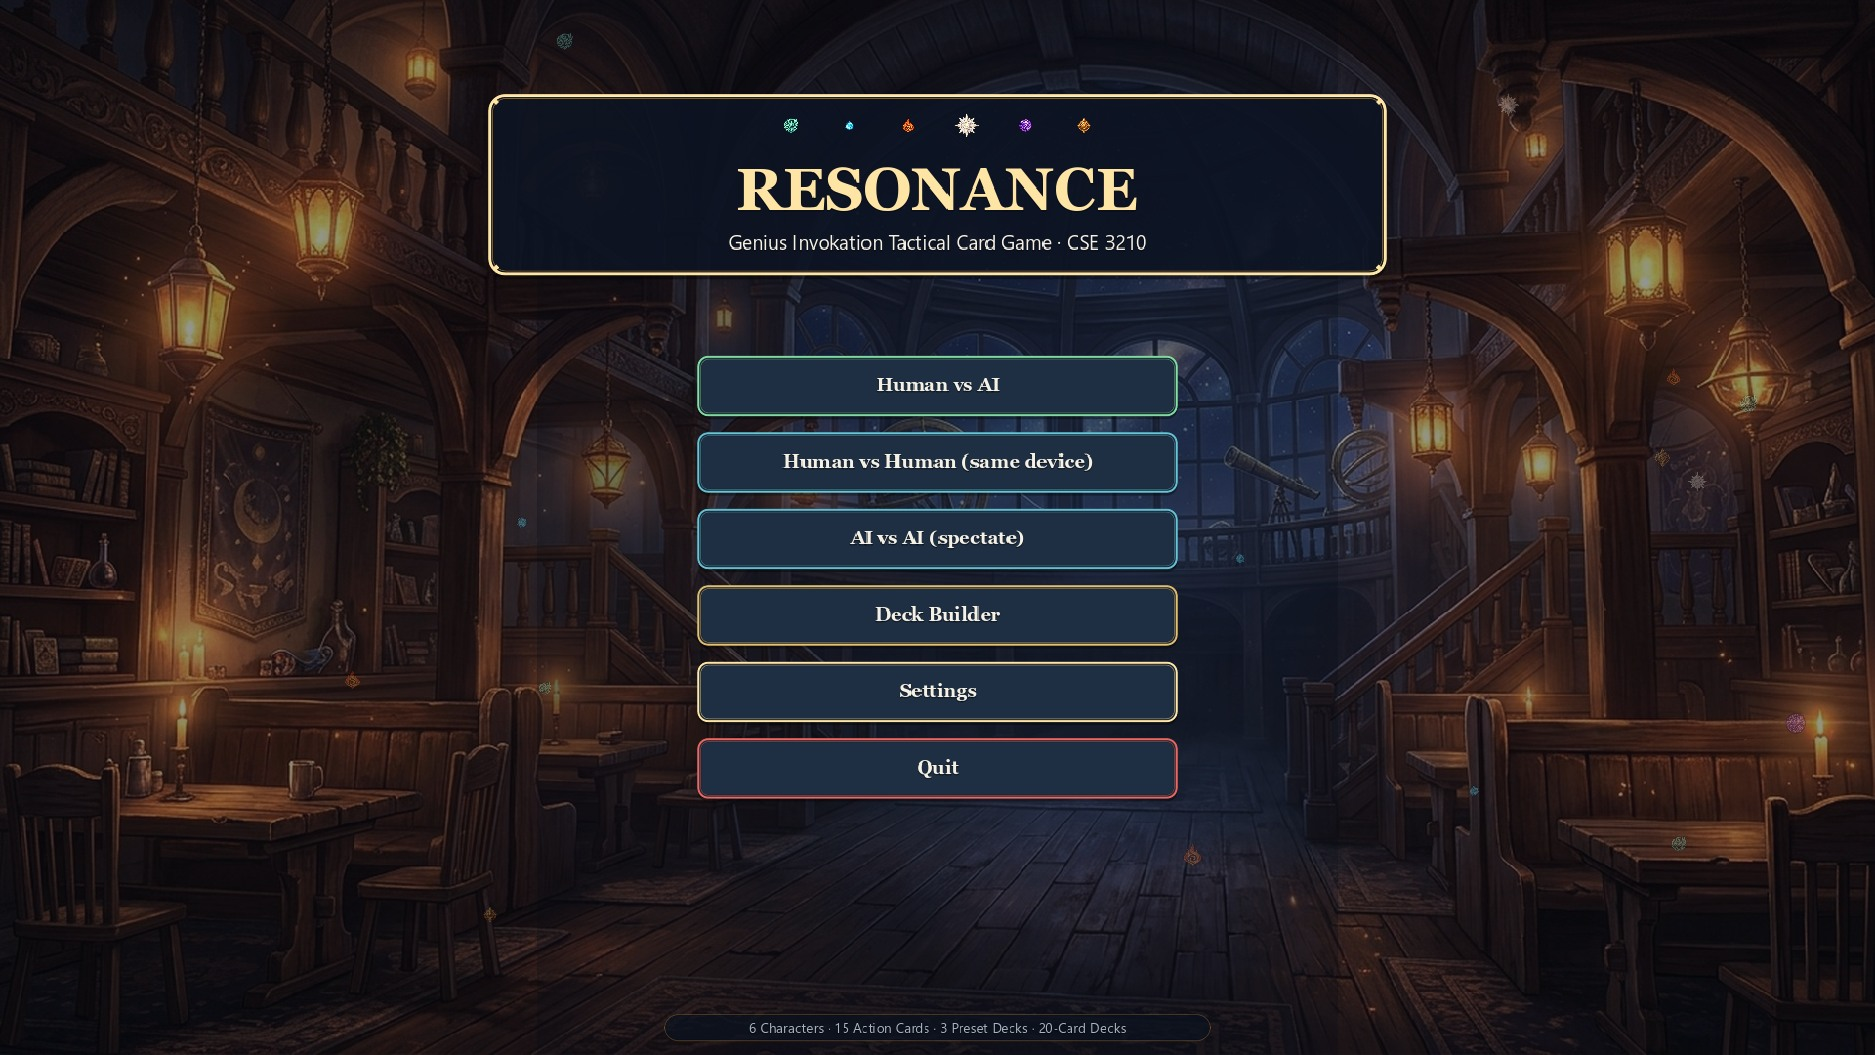
\includegraphics[width=\textwidth]{images/ui_main_menu.jpg}
  \caption{Main Menu with mode selection, Deck Builder, and Settings.}
\end{subfigure}\hfill
\begin{subfigure}[b]{0.485\textwidth}
  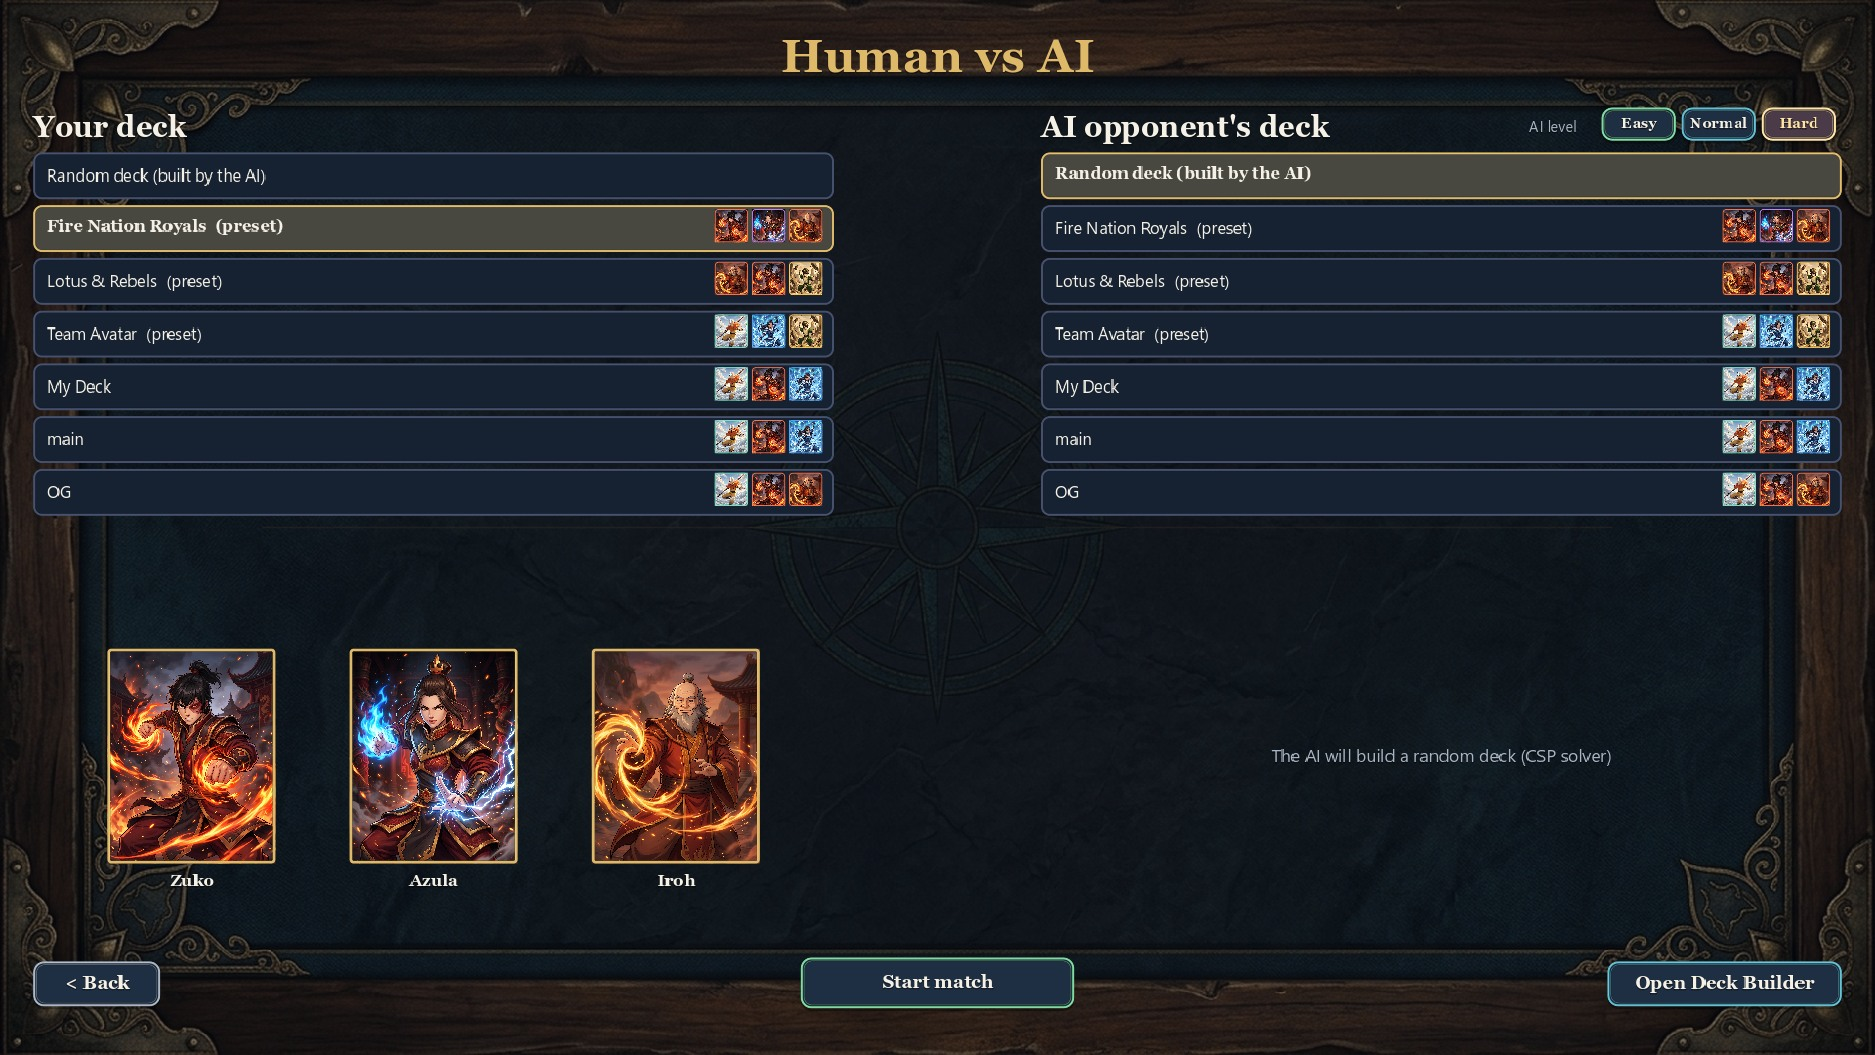
\includegraphics[width=\textwidth]{images/ui_deck_select.jpg}
  \caption{Pre-match setup: preset/custom decks, AI tier, and CSP random deck option.}
\end{subfigure}
\caption{Entry and pre-match configuration screens.}
\label{fig:ui-menu-select}
\end{figure}

\begin{figure}[H]
\centering
\begin{subfigure}[b]{0.485\textwidth}
  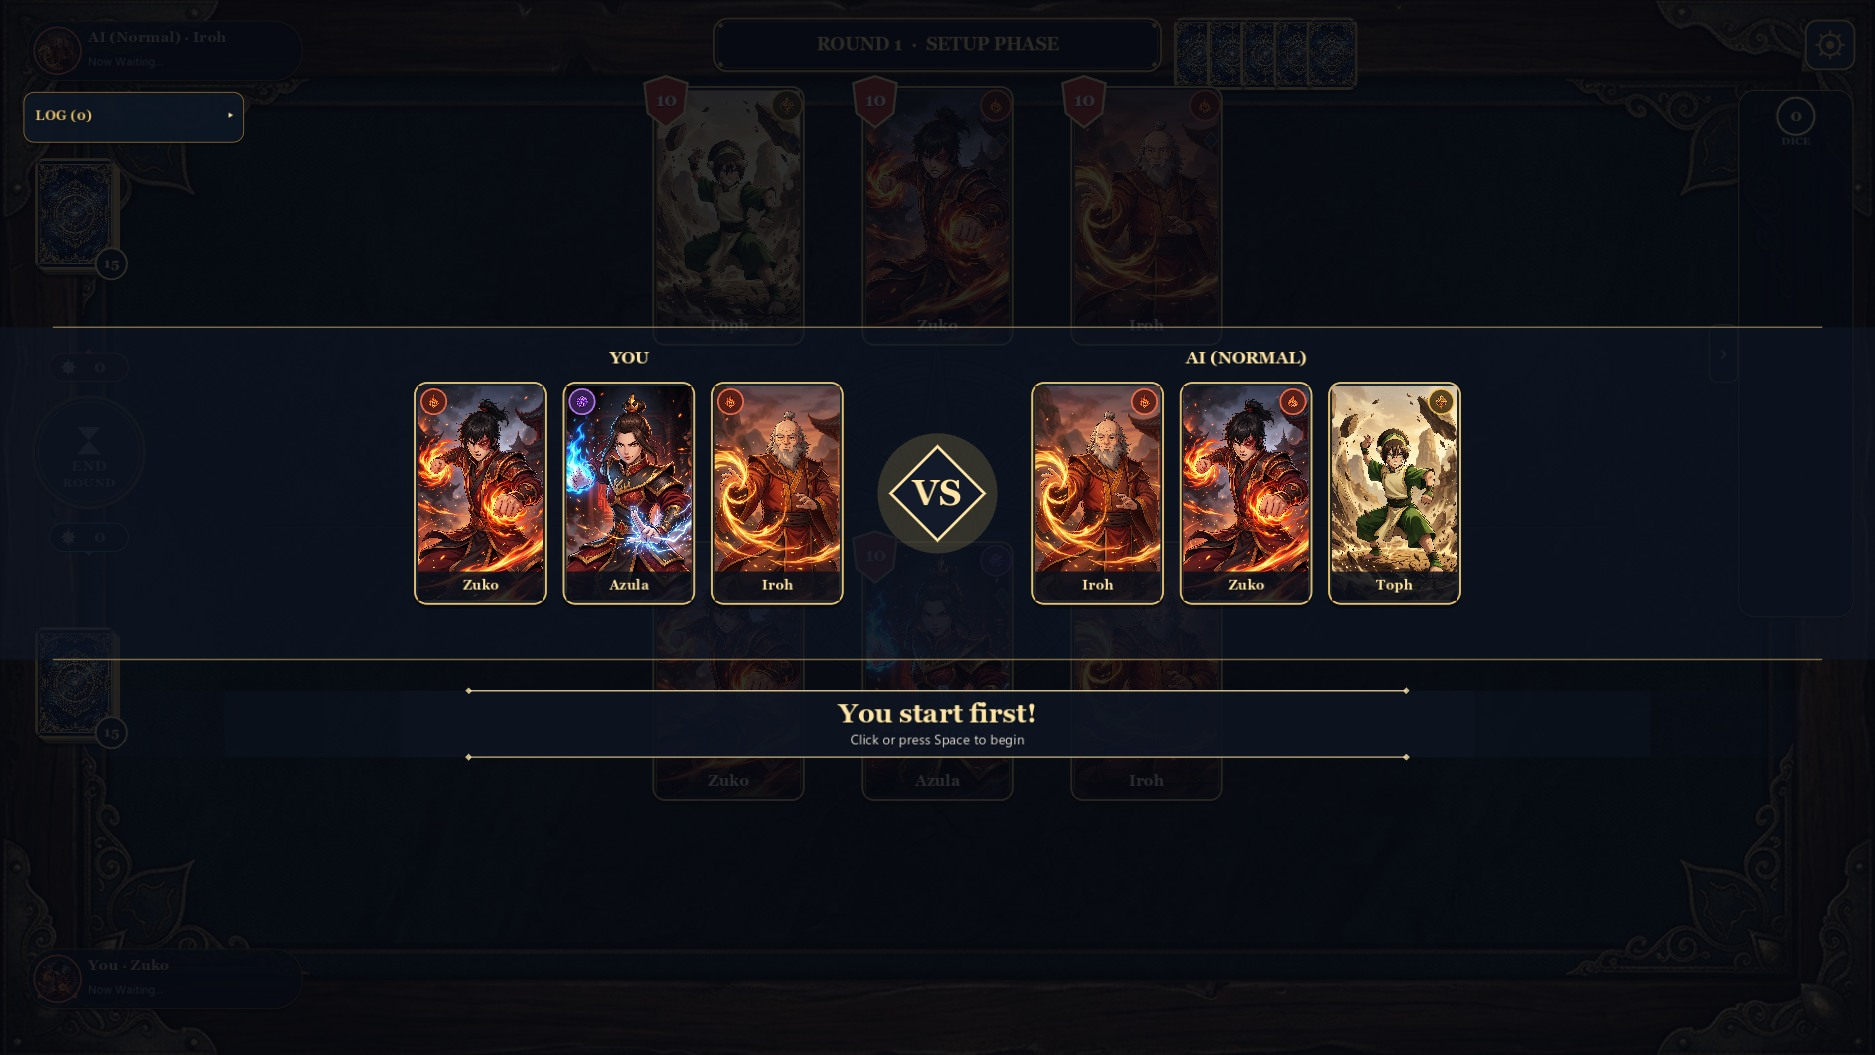
\includegraphics[width=\textwidth]{images/ui_vs_intro.jpg}
  \caption{Opening VS lineup and coin-toss initiative announcement.}
\end{subfigure}\hfill
\begin{subfigure}[b]{0.485\textwidth}
  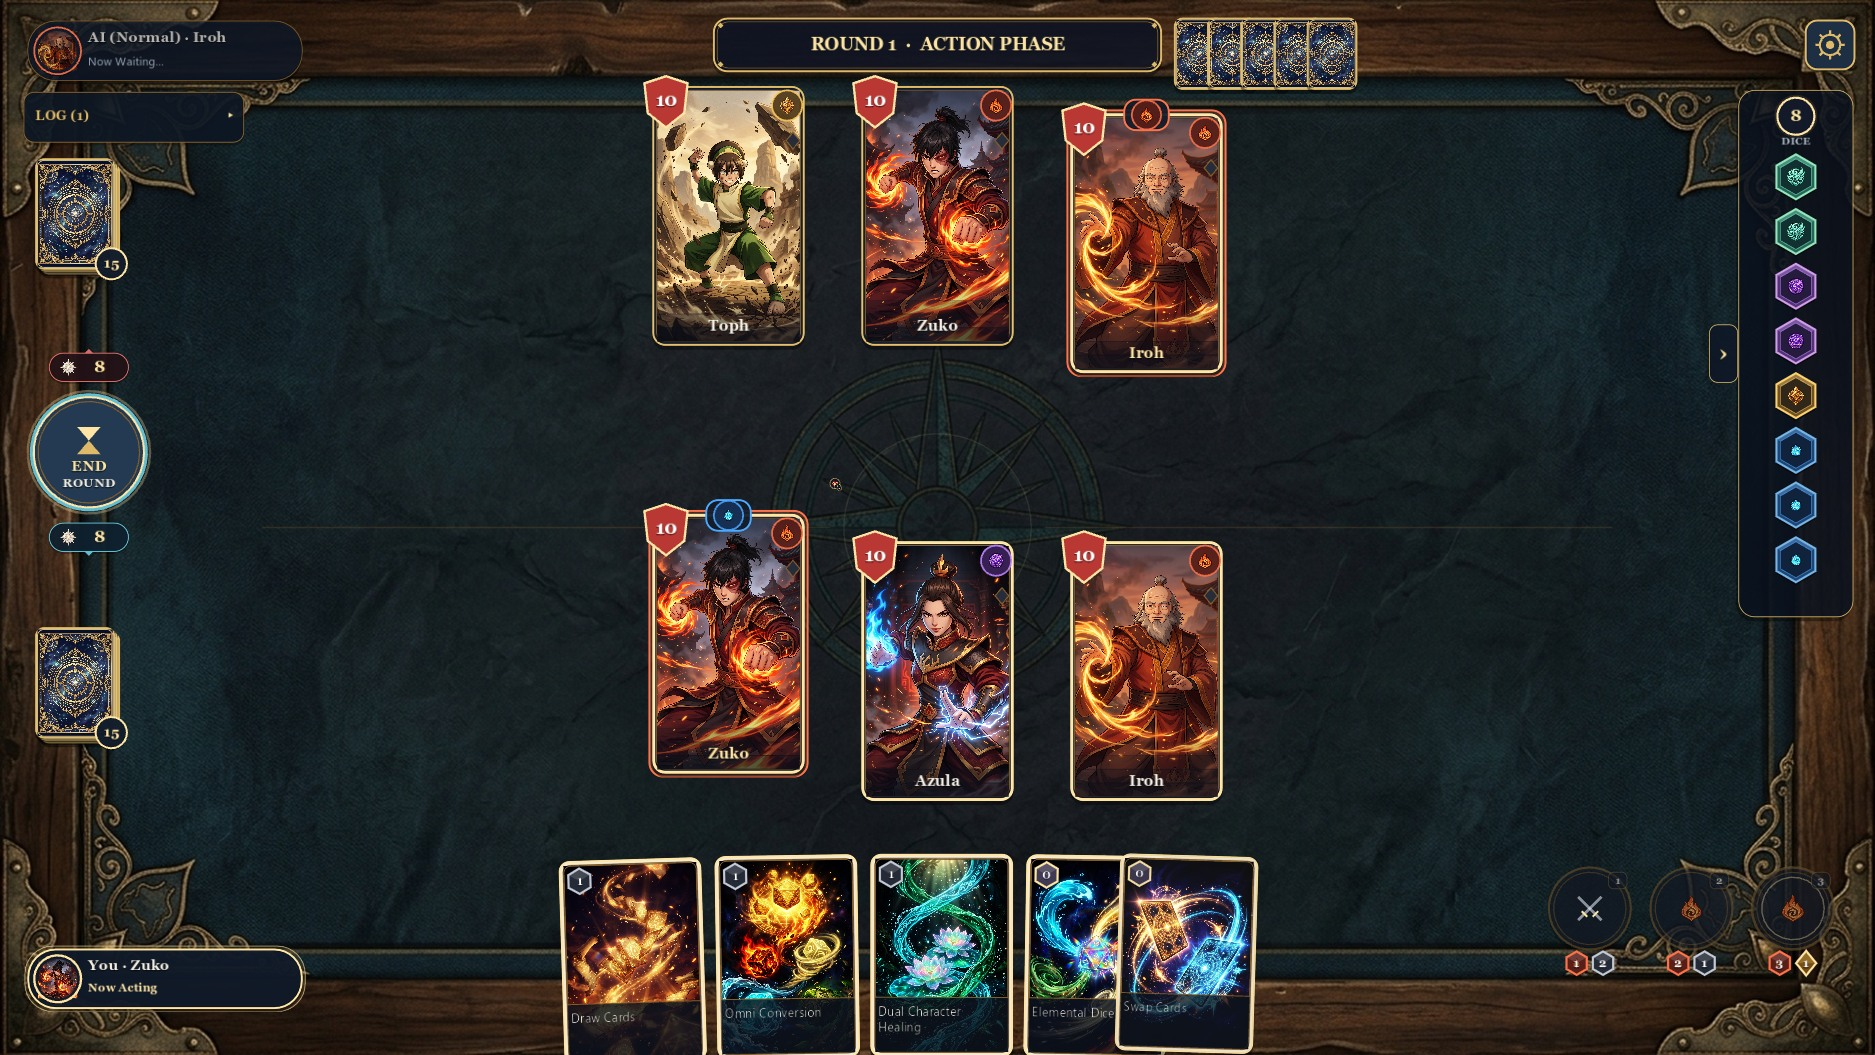
\includegraphics[width=\textwidth]{images/ui_board_action.jpg}
  \caption{Action Phase tabletop: active units, hand fan, 8-dice tray, and End Round hourglass.}
\end{subfigure}
\caption{Match start presentation and live Action Phase board.}
\label{fig:ui-intro-board}
\end{figure}

\begin{figure}[H]
\centering
\begin{subfigure}[b]{0.485\textwidth}
  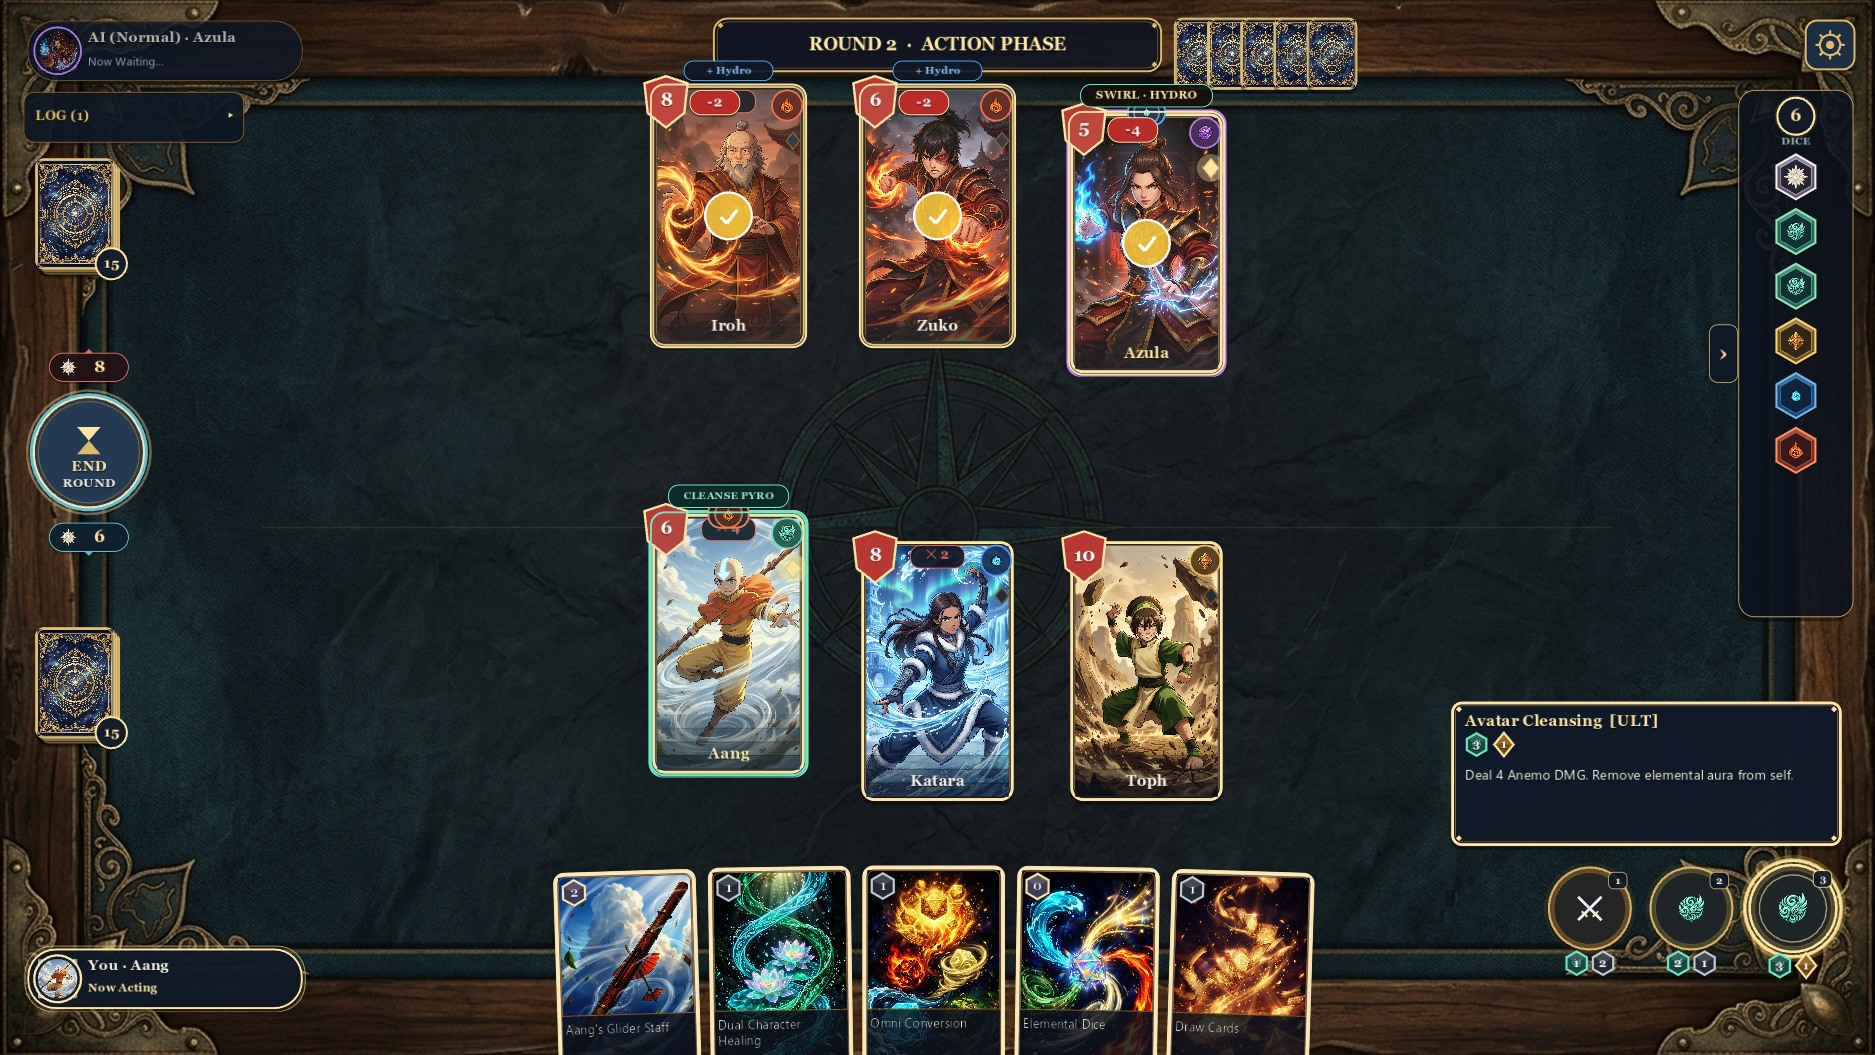
\includegraphics[width=\textwidth]{images/ui_skill_preview.jpg}
  \caption{Click-1 forecast for Aang's \emph{Avatar Cleansing}: \texttt{-4} Swirl on Azula, \texttt{-2 +Hydro} on Zuko \& Iroh, and \texttt{CLEANSE PYRO} on Aang.}
\end{subfigure}\hfill
\begin{subfigure}[b]{0.485\textwidth}
  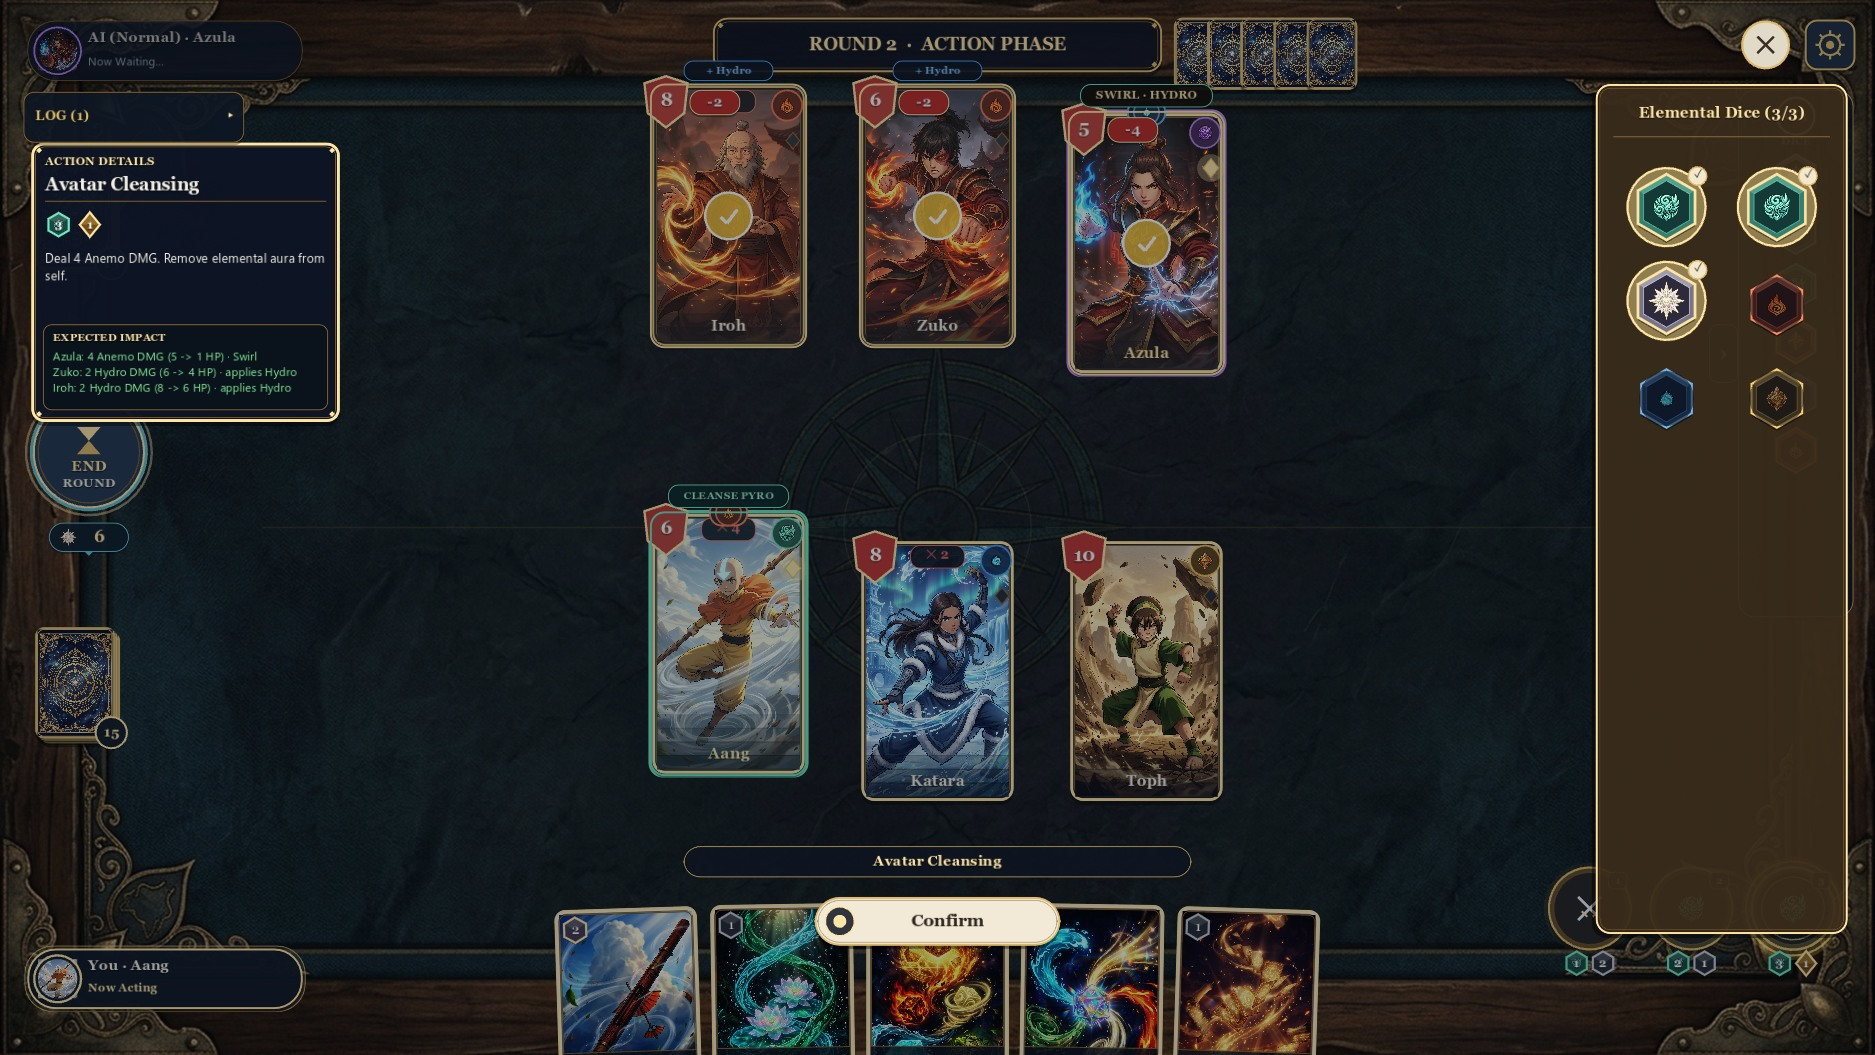
\includegraphics[width=\textwidth]{images/ui_inline_payment.jpg}
  \caption{Click-2 inline dice payment with Expected Impact panel, highlighted 3/3 dice, Confirm pill, and non-overlapping Cancel button.}
\end{subfigure}
\caption{Two-step skill preview and inline dice payment on the exact Round~2 position analyzed in Section~\ref{sec:tree}.}
\label{fig:ui-preview-pay}
\end{figure}

\begin{figure}[H]
\centering
\begin{subfigure}[b]{0.485\textwidth}
  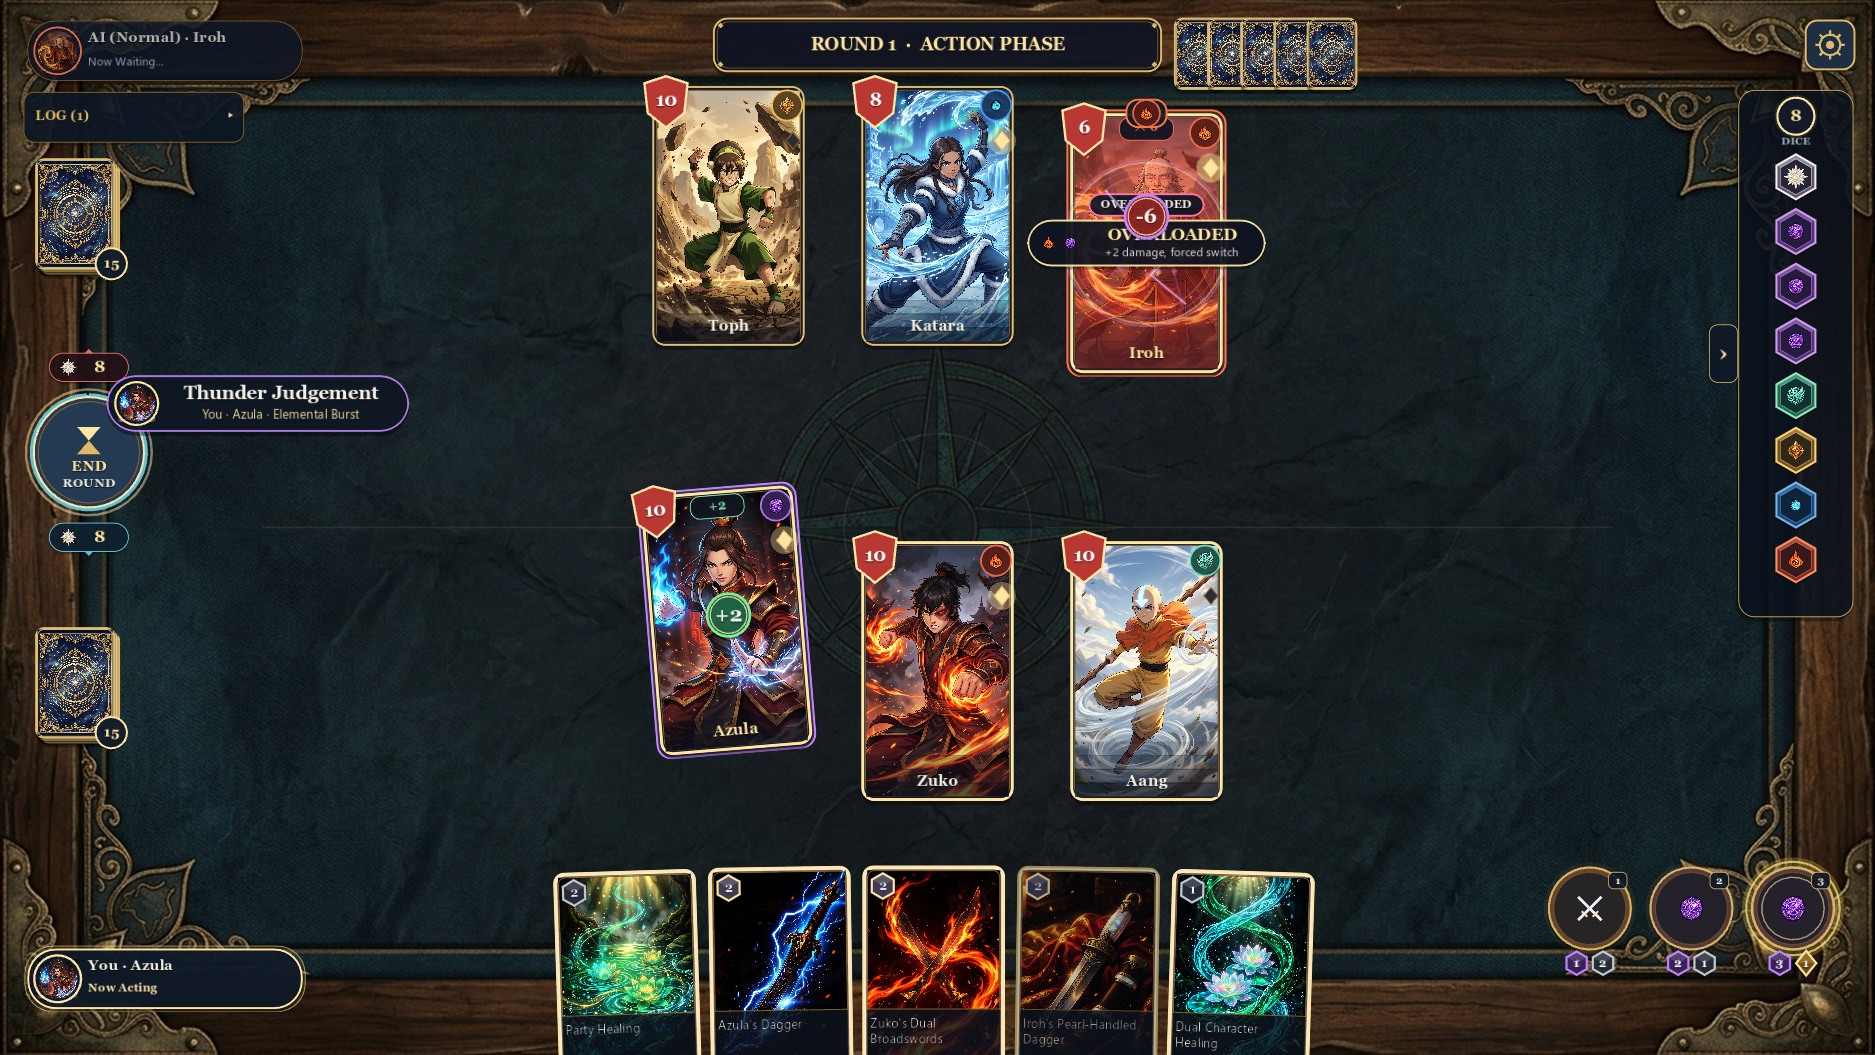
\includegraphics[width=\textwidth]{images/ui_combat_reaction.jpg}
  \caption{Elemental Burst announcement ribbon (\emph{Thunder Judgement}) and \emph{Overloaded} reaction VFX.}
\end{subfigure}\hfill
\begin{subfigure}[b]{0.485\textwidth}
  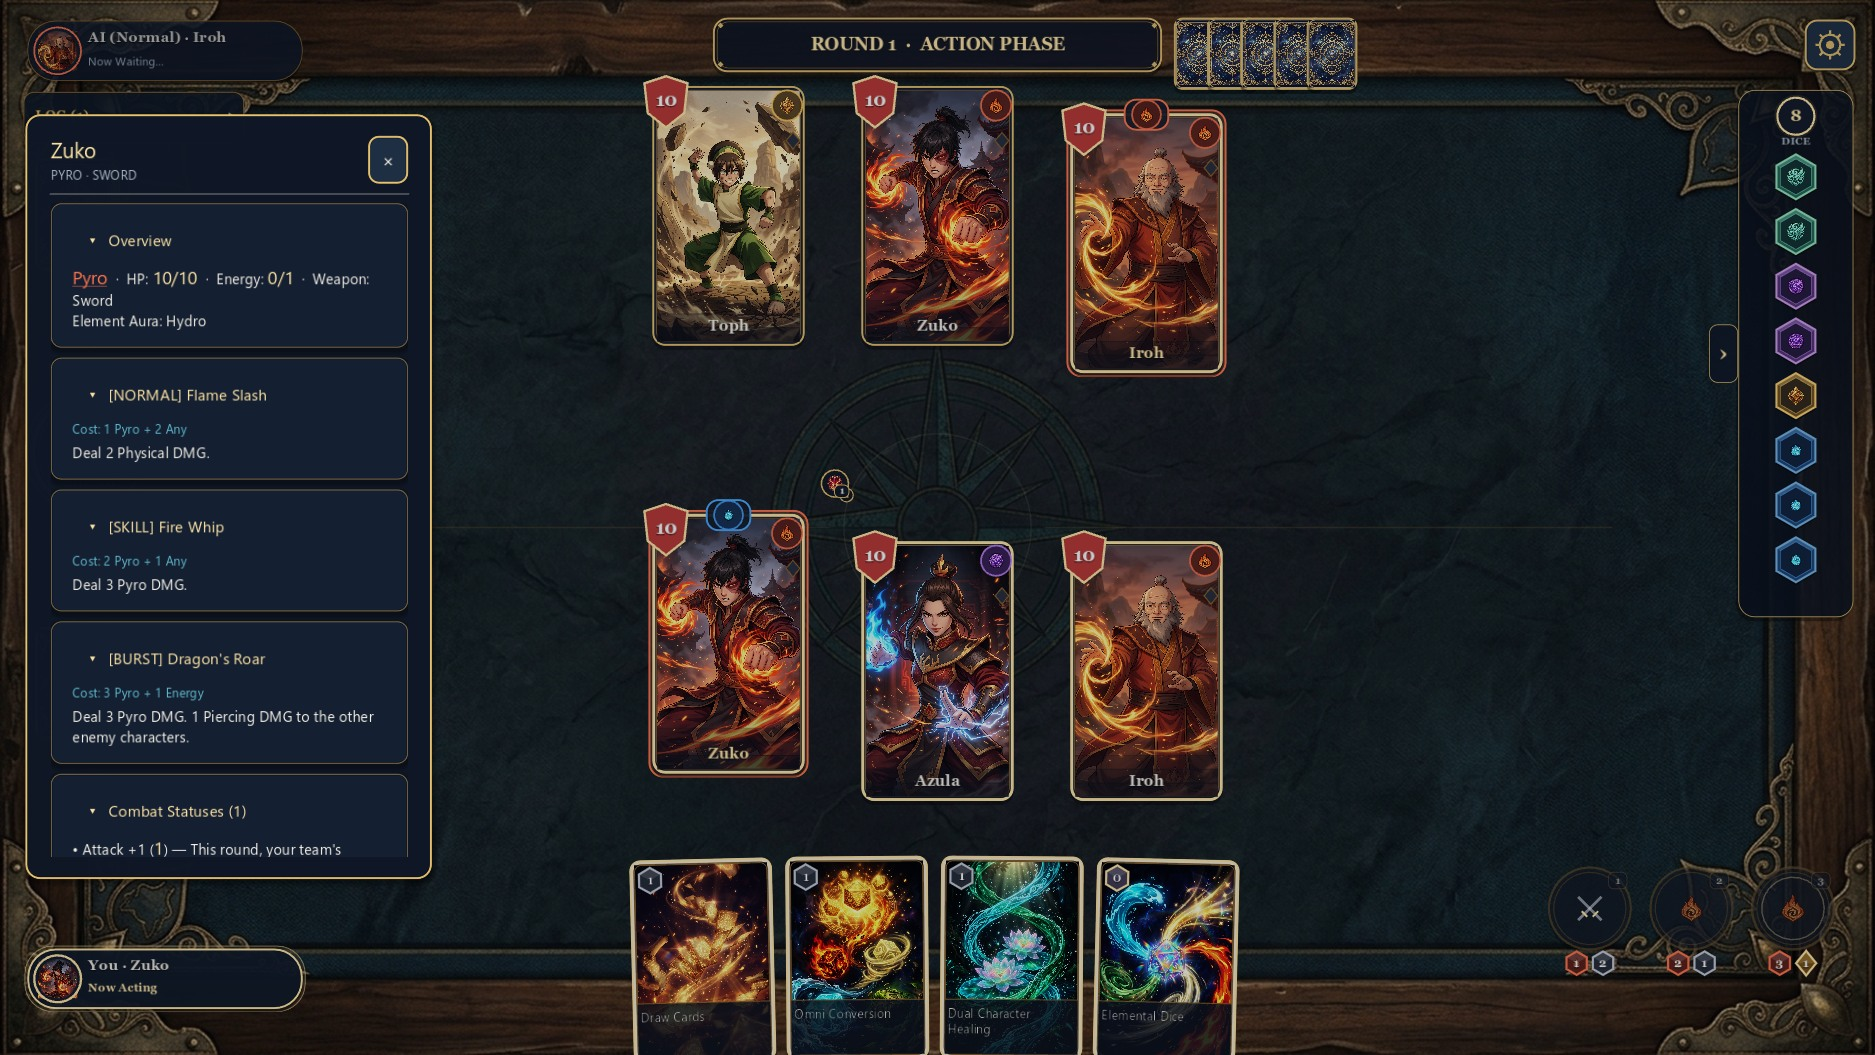
\includegraphics[width=\textwidth]{images/ui_inspect_drawer.jpg}
  \caption{Character Inspector drawer displaying stats, active aura, skills, and team combat statuses.}
\end{subfigure}

\vspace{0.25cm}
\begin{subfigure}[b]{0.485\textwidth}
  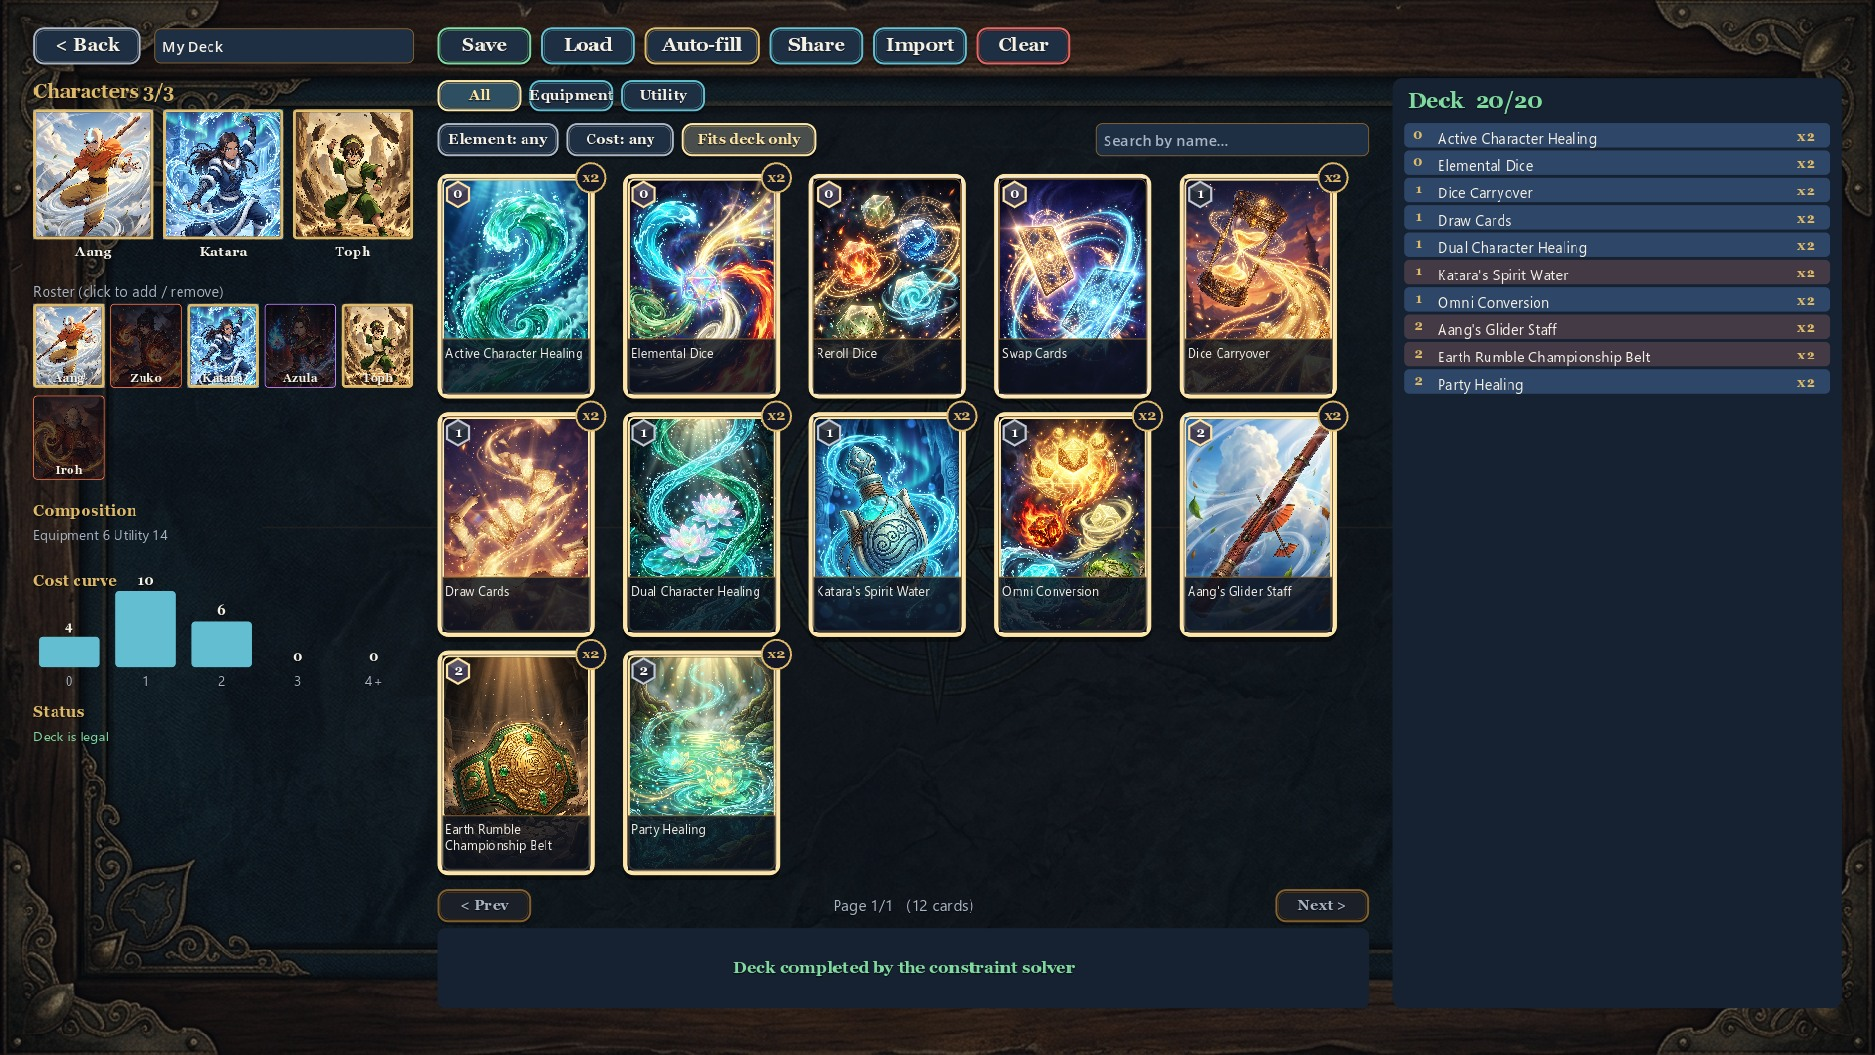
\includegraphics[width=\textwidth]{images/ui_deck_builder.jpg}
  \caption{Deck Builder showing 20/20 Team Avatar deck, cost curve, and CSP Auto-fill confirmation.}
\end{subfigure}\hfill
\begin{subfigure}[b]{0.485\textwidth}
  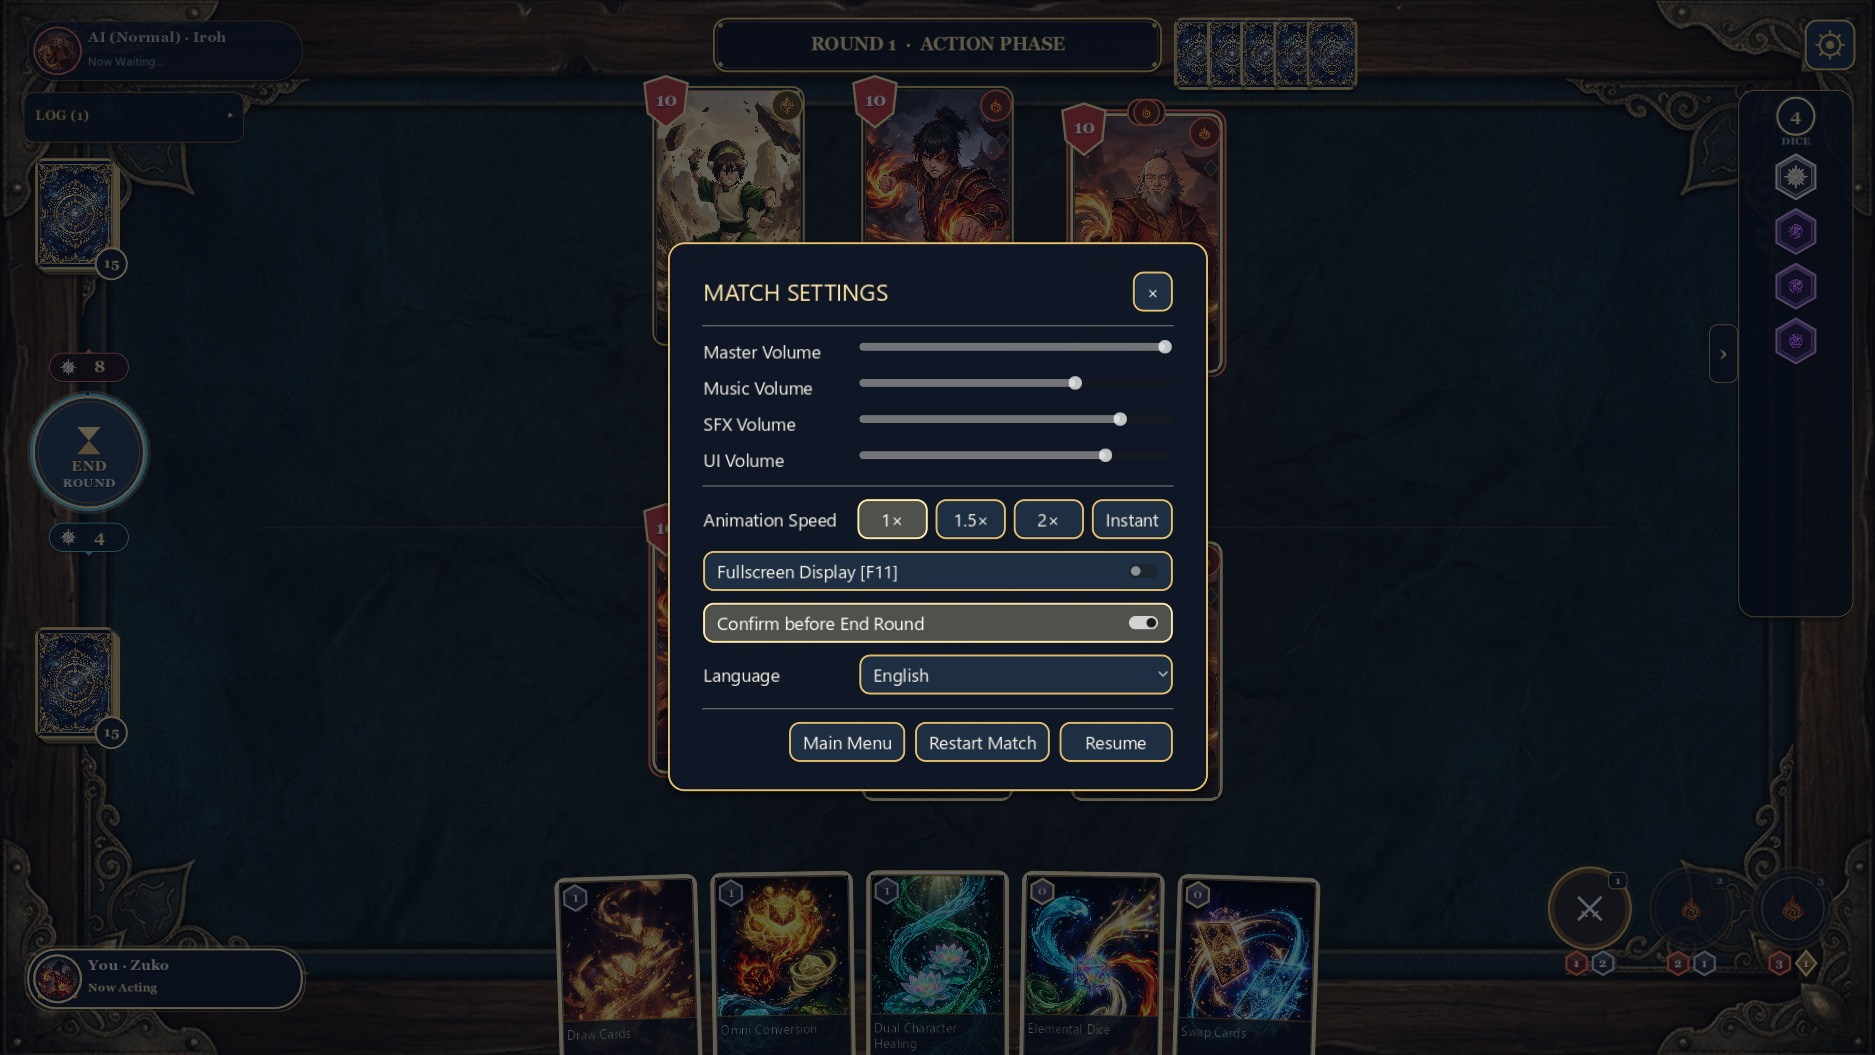
\includegraphics[width=\textwidth]{images/ui_settings_modal.jpg}
  \caption{Match Settings modal: audio buses, animation speed, Fullscreen \texttt{[F11]}, and End Round confirmation.}
\end{subfigure}
\caption{Combat feedback, inspection, CSP deck building, and live settings controls.}
\label{fig:ui-gallery}
\end{figure}

% ==============================================================================
% SECTION 7: ALGORITHMS
% ==============================================================================
\section{Algorithms}

All three AI tiers share a common entry point \texttt{TCGAIPlayer.choose(state)} that never mutates the input state. In Setup, the AI mulligans expensive ($\ge 4$ cost) or duplicate equipment cards and opens with the lowest-energy character that has elemental reaction partners. In Roll Phase, it rerolls all non-matching, non-Omni dice. During the Action Phase, it runs a six-stage pipeline:
{\small
\[
  \text{Fuzzy Profile} \;\to\; \text{1-Die Tune} \;\to\; \text{Determinize} \;\to\; \text{A* Lethal} \;\to\; \text{Tier Search} \;\to\; \text{CSP Smart Pay}.
\]}

\subsection{Determinization, Pre-Search Tuning, and Move Ordering}

\textbf{Imperfect-Information Determinization (\texttt{TCGWorld.determinize}).} To guarantee strict fairness (zero cheating), the AI never inspects the opponent's true hand or either deck order. Before searching, it clones the state, constructs a legal pool of two copies of every card permitted for the opponent's three characters, shuffles that pool, deals $|H_{\text{foe}}|$ sampled cards into the opponent's hand and $|K_{\text{foe}}|$ into their deck, and shuffles its own remaining deck.

\textbf{Pre-Search Elemental Tuning.} If the active character is not stunned and cannot currently cast an Elemental Skill or Burst, \texttt{\_tune} checks whether any Skill or Burst is \emph{exactly one aligned die short} while total dice suffice. If so, the AI immediately converts one off-element die by discarding its least-useful card (preferring high-cost Events over Equipment).

\textbf{Move Ordering and Opponent-Card Pruning (\texttt{TCGWorld.candidates}).} To eliminate redundant branching during search, tuning actions are excluded from inner search nodes (handled upfront by \texttt{\_tune}), and opponent \texttt{card} actions are omitted so search never hallucinates reactions to randomly sampled opponent cards. Remaining legal moves are sorted by priority:
\[
  \texttt{choose\_active},\;\texttt{skill}\;(\text{Burst} \succ \text{Skill} \succ \text{Normal}) \;\succ\; \texttt{card} \;\succ\; \texttt{switch} \;\succ\; \texttt{end\_round}.
\]
Ordering high-impact skills first dramatically improves Alpha-Beta cutoff rates.

\subsection{Sugeno Fuzzy Logic Profiler and Evaluation Function}

\textbf{Sugeno Fuzzy Style Profiler (\texttt{TCGFuzzy}).} Rather than keeping static evaluation weights across every match phase, the AI computes six normalized state features in $[0,1]$ (with $\text{dice}$ capped at $1.5$):
\[
  x = \Big(\text{hp}_{\text{me}},\; \text{hp}_{\text{foe}},\; \text{en}_{\text{me}},\; \text{en}_{\text{foe}},\; \min(\tfrac{|D_{\text{me}}|}{8}, 1.5),\; \tfrac{|H_{\text{me}}|}{10}\Big).
\]
Each feature maps into three trapezoidal linguistic sets using $\mathrm{trap}(x; a,b,c,d)$:
\begin{equation}
  \begin{aligned}
    \mu_{\text{low}}(x)  &= \mathrm{trap}(x; -1, -1, 0.25, 0.55), \qquad
    \mu_{\text{med}}(x)  = \mathrm{trap}(x; 0.25, 0.50, 0.50, 0.75), \\
    \mu_{\text{high}}(x) &= \mathrm{trap}(x; 0.45, 0.75, 2.0, 2.0).
  \end{aligned}
\end{equation}
Five zero-order Sugeno rule bases compute crisp playing-style scalars via weighted average $\frac{\sum_j w_j o_j}{\sum_j w_j}$ (for example, $\text{defence}$ fires on $\mu_{\text{low}}(\text{hp}_{\text{me}}) \Rightarrow 0.90$, $\mu_{\text{med}}(\text{hp}_{\text{me}}) \Rightarrow 0.50$, $\mu_{\text{high}}(\text{hp}_{\text{me}}) \Rightarrow 0.15$, and $\mu_{\text{high}}(\text{en}_{\text{foe}}) \Rightarrow 0.80$; $\text{burst}$ fires on $\mu_{\text{high}}(\text{en}_{\text{me}}) \Rightarrow 0.95$, $\mu_{\text{med}} \Rightarrow 0.50$, $\mu_{\text{low}} \Rightarrow 0.15$). These dynamically adapt the heuristic evaluation weights:
\begin{equation}
  w_{\text{hp}} = 0.8 + 0.6 \cdot \text{defence}, \qquad
  w_{\text{energy}} = 0.8 + 0.6 \cdot \text{burst}, \qquad
  w_{\text{board}} = 1.0.
\end{equation}

\textbf{Heuristic Evaluation Function (\texttt{TCGEvaluate}).} For terminal states, $\fn{Eval}(s) = +6.0$ (win), $-6.0$ (loss), or $0.0$ (draw). For non-terminal states, the function is strictly zero-sum:
\begin{equation}
  \fn{Eval}(s, \text{me}) = \fn{Side}(P_{\text{me}}, P_{\text{foe}}) - \fn{Side}(P_{\text{foe}}, P_{\text{me}}),
  \label{eq:eval}
\end{equation}
where $\fn{Side}(P, Q)$ sums the material, energy, status, and resource terms detailed in Table~\ref{tab:eval-weights}.

\begin{table}[H]
\centering
\caption{Components of $\fn{Side}(P, Q)$ in the fuzzy-weighted evaluation function (Equation~\ref{eq:eval}).}
\label{tab:eval-weights}
\small
\begin{tabularx}{\textwidth}{@{}L{3.2cm} L{6.2cm} Y@{}}
\toprule
Term & Formula / Weight & Tactical Justification \\
\midrule
Living character base & $+0.45$ per alive unit & Preserving bodies prevents defeat and keeps elements. \\
Health ratio & $+0.70 \cdot w_{\text{hp}} \cdot (\text{hp}_c / \text{hp}_{\max})$ & Scales HP value up when hurt or facing Burst energy. \\
Energy charge & $+w_{\text{energy}} \cdot (\text{en}_c / \text{en}_{\max}) \cdot (0.25 \text{ active},\, 0.12 \text{ bench})$ & Values charged Ultimates twice as much when active. \\
Equipment bonus & $+0.07$ per equipped item & Rewards persistent $+1$~DMG weapons and \emph{Spirit Water}. \\
Aura vulnerability & $-0.08 \cdot (0.5 + w_{\text{defence}})$ if foe can react & Penalizes exposed auras (motivates cleansing). \\
Crowd control & $-0.22$ if \emph{Stunned}/\emph{Frozen}/\emph{Petrified} & Penalizes inability to cast skills until End Phase. \\
Combat statuses & $+0.06 \cdot (\text{shield} + 0.5 \cdot \max(0,\text{usages}))$ & Values \emph{Shield +2}, \emph{Crystallize}, and round buffs. \\
Hand \& Action dice & $+0.02 |H| + 0.012 |D|$ (Action Phase only) & Small tie-breaker favoring card and dice efficiency. \\
\bottomrule
\end{tabularx}
\end{table}

\subsection{Informed A* Lethal Planner}

Before running deep adversarial search, both \emph{Normal} and \emph{Hard} invoke \texttt{TCGPlanner.plan\_lethal} (Algorithm~\ref{alg:astar}) to check whether a sequence of actions within the \emph{current turn} can immediately defeat the opponent's active character (or win the match) at minimal dice and card cost.

Each search node has path cost $g(n) = (|D_0| - |D|) + 0.3(|H_0| - |H|) + 0.05 \cdot (\text{steps}-1)$ and heuristic
\begin{equation}
  h(n) = \max\!\left(0,\; \frac{\text{HP}_{\text{target}}}{2.5} - 0.5\right), \qquad f(n) = g(n) + h(n).
  \label{eq:astar-h}
\end{equation}
Because even buffed Burst + Reaction combos rarely exceed 2.5 damage per die spent, $h(n)$ stays optimistic (admissible), ensuring A* returns the cheapest single-turn knockout sequence. Crucially, the planner empties the AI's own deck inside its cloned root state $s_0$ so it never relies on lucky unseen draws.

\begin{algorithm}[H]
\caption{Single-Turn Informed A* Lethal Planner (\texttt{TCGPlanner.plan\_lethal})}
\label{alg:astar}
\small
\begin{algorithmic}[1]
\Function{PlanLethal}{$s, \text{me}, B_{\max}=250$}
  \State $t \gets s.\text{players}[1-\text{me}].\text{active}$; \quad $s_0 \gets \fn{Clone}(s)$;\quad $s_0.\text{players}[\text{me}].\text{deck} \gets \emptyset$
  \State $\text{open} \gets \{(\fn{h}(s_0, t),\, 0,\, s_0,\, [\,])\}$; \quad $\text{seen} \gets \emptyset$; \quad $\text{exp} \gets 0$
  \While{$\text{open} \neq \emptyset$ \textbf{and} $\text{exp} < B_{\max}$}
    \State $(f, g, u, \pi) \gets \fn{PopMin}(\text{open})$ \Comment{lowest $f$, tie-break by lowest $g$}
    \If{$\pi \neq [\,]$ \textbf{and} ($u.\text{players}[1-\text{me}].\text{chars}[t].\text{defeated}$ \textbf{or} $u.\text{winner} = \text{me}$)}
      \State \Return $\pi$ \Comment{cheapest guaranteed lethal sequence}
    \EndIf
    \If{$\fn{Player}(u) \neq \text{me}$ \textbf{or} $u.\text{phase} \neq \text{action}$ \textbf{or} $u.\text{winner} \neq -2$}
      \State \textbf{continue} \Comment{turn ended without knockout: dead end}
    \EndIf
    \State $\text{exp} \gets \text{exp} + 1$
    \ForAll{$a \in \fn{Candidates}(u, \text{me})$ with $a.\text{type} \neq \texttt{end\_round}$}
      \State $u' \gets \fn{Result}(\fn{Clone}(u), a)$;\quad $k \gets \fn{StateKey}(u', \text{me})$
      \If{$k \notin \text{seen}$}
        \State $\text{seen} \gets \text{seen} \cup \{k\}$;\quad $g' \gets \fn{Spent}(s_0, u') + 0.05|\pi|$
        \State $\fn{Push}(\text{open},\, (g' + \fn{h}(u', t),\, g',\, u',\, \pi \mathbin{\Vert} [a]))$
      \EndIf
    \EndFor
  \EndWhile
  \State \Return $\text{null}$
\EndFunction
\end{algorithmic}
\end{algorithm}
\textbf{Symbols.} $t$ = opponent's active character index; $B_{\max}=250$ = expansion cap; $\pi$ = action sequence from $s_0$; $\fn{Spent}(s_0,u') = \Delta |D| + 0.3\Delta|H|$ = dice and card resources spent; $\fn{h}(u',t)$ = Equation~\ref{eq:astar-h}; $\fn{StateKey}$ hashes sorted dice, sorted hand, enemy HP vector, and active index.

\subsection{Agent 1 (Normal): Iterative-Deepening Alpha-Beta Search}

If no immediate knockout exists, \emph{Normal} runs Iterative-Deepening Minimax with Alpha-Beta pruning (\texttt{TCGSearcher}, Algorithm~\ref{alg:ab}). As illustrated in Figure~\ref{fig:ab-concept}, MAX maintains lower bound $\alpha$ and MIN maintains upper bound $\beta$; whenever $\beta \le \alpha$, the remaining siblings cannot affect the root choice and are pruned immediately.

Two domain-specific adjustments make Alpha-Beta accurate for a TCG:
\begin{enumerate}[leftmargin=1.4em, itemsep=1pt]
  \item \textbf{Zero Depth Cost for Fast Actions:} $\fn{Cost}(a) = 1$ for Combat Actions (\texttt{skill}, \texttt{switch}, \texttt{end\_round}) and $\fn{Cost}(a) = 0$ for Fast Actions (\texttt{card}, \texttt{choose\_active}). Thus playing a 0-cost card never pushes the opponent's reply beyond the search horizon.
  \item \textbf{End-Round Tempo Penalty:} Ending the round adds $\fn{EndPenalty}(s, a) = \pm(b_{\text{first}} - 0.014|D|(1.5 - \text{tempo}))$, where $b_{\text{first}} = 0.03$ if ending first (securing next-round initiative) and $-0.014|D|(1.5-\text{tempo})$ penalizes wasting unspent dice.
\end{enumerate}

\begin{figure}[H]
\centering
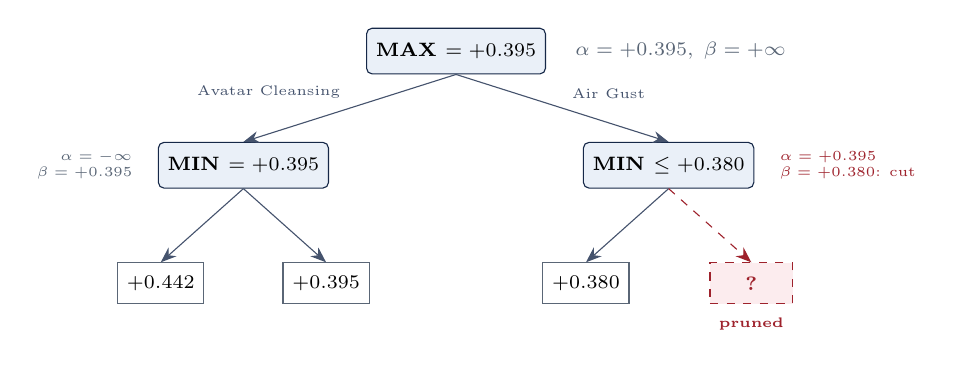
\begin{tikzpicture}[
  lvl/.style={rectangle, rounded corners=2pt, draw=navy, fill=softblue, minimum width=2.05cm, minimum height=0.58cm, font=\scriptsize\bfseries},
  leaf/.style={rectangle, draw=slate, fill=white, minimum width=1.05cm, minimum height=0.52cm, font=\scriptsize\bfseries},
  cut/.style={rectangle, dashed, draw=crimson, fill=softred, minimum width=1.05cm, minimum height=0.52cm, font=\scriptsize\bfseries, text=crimson},
  edge/.style={-{Stealth[length=2mm]}, color=navy!80}
]
  \node[lvl] (root) at (0,0) {MAX $= +0.395$};
  \node[right=0.25cm of root, font=\scriptsize, color=slate] {$\alpha = +0.395,\; \beta = +\infty$};
  \node[lvl] (m1) at (-2.7,-1.45) {MIN $= +0.395$};
  \node[lvl] (m2) at (2.7,-1.45) {MIN $\le +0.380$};
  \node[left=0.2cm of m1, font=\tiny, color=slate, align=right] {$\alpha=-\infty$\\$\beta=+0.395$};
  \node[right=0.2cm of m2, font=\tiny, color=crimson, align=left] {$\alpha=+0.395$\\$\beta=+0.380$: cut};
  \node[leaf] (l1) at (-3.75,-2.95) {$+0.442$};
  \node[leaf] (l2) at (-1.65,-2.95) {$+0.395$};
  \node[leaf] (l3) at (1.65,-2.95) {$+0.380$};
  \node[cut]  (l4) at (3.75,-2.95) {?};
  \node[below=0.05cm of l4, font=\tiny\bfseries, color=crimson] {pruned};
  \draw[edge] (root.south) -- node[above left, font=\tiny] {Avatar Cleansing} (m1.north);
  \draw[edge] (root.south) -- node[above right, font=\tiny] {Air Gust} (m2.north);
  \draw[edge] (m1.south) -- (l1.north);
  \draw[edge] (m1.south) -- (l2.north);
  \draw[edge] (m2.south) -- (l3.north);
  \draw[edge, dashed, crimson] (m2.south) -- (l4.north);
\end{tikzpicture}
\caption{Alpha-Beta pruning on a slice of our real Round~2 tree: once \emph{Air Gust}'s first reply yields $+0.380 \le \alpha = +0.395$, all remaining replies are skipped.}
\label{fig:ab-concept}
\end{figure}

\begin{algorithm}[H]
\caption{Iterative-Deepening Alpha-Beta Search (\texttt{TCGSearcher})}
\label{alg:ab}
\small
\begin{algorithmic}[1]
\Function{AlphaBeta}{$s, d, \alpha, \beta$}
  \State $\text{nodes} \gets \text{nodes} + 1$
  \If{$d \le 0$ \textbf{or} $\fn{Terminal}(s)$ \textbf{or} ($s.\text{phase} \neq \text{action}$ \textbf{and} $s.\text{pending}=\emptyset$)}
    \State \Return $\fn{Eval}(s, \text{me}, \text{prof})$ \Comment{Equation~\ref{eq:eval}}
  \EndIf
  \If{$\text{nodes} > N_{\max}$ \textbf{or} $\fn{TimeNow}() > t_{\text{deadline}}$}
    \State $\text{aborted} \gets \text{true}$; \quad \Return $\fn{Eval}(s, \text{me}, \text{prof})$
  \EndIf
  \State $\text{maximizing} \gets (\fn{Player}(s) = \text{me})$;\quad $v \gets -\infty$ \textbf{if} maximizing \textbf{else} $+\infty$
  \ForAll{$a \in \fn{Candidates}(s, \text{me})$}
    \State $c \gets \fn{Result}(\fn{Clone}(s), a)$
    \State $v' \gets \fn{AlphaBeta}(c,\, d - \fn{Cost}(a),\, \alpha,\, \beta) + \fn{EndPenalty}(s, a)$
    \If{maximizing}
      \State $v \gets \max(v, v')$;\quad $\alpha \gets \max(\alpha, v)$
    \Else
      \State $v \gets \min(v, v')$;\quad $\beta \gets \min(\beta, v)$
    \EndIf
    \If{$\beta \le \alpha$ \textbf{or} $\text{aborted}$} \textbf{break} \Comment{alpha-beta cutoff} \EndIf
  \EndFor
  \State \Return $v$
\EndFunction
\end{algorithmic}
\end{algorithm}
\textbf{Symbols.} $d$ = remaining turn-ending plies (iterative deepening $d = 1,2,3,4$); $N_{\max}=6000$ nodes, $t_{\text{deadline}}=0.6\text{ s}$ on Normal; $\fn{Cost}(a) \in \{0,1\}$; $\text{prof}$ = Sugeno fuzzy profile. After each completed depth $d$, root moves are re-sorted by score so depth $d+1$ explores the principal variation first; if a deeper pass aborts, the last fully completed depth's move is kept.

\subsection{Agent 2 (Hard): Shortlisted Information-Set MCTS}

\emph{Hard} combines tactical pruning with stochastic look-ahead across hidden information. First, it allocates 35\% of its time budget ($0.56\text{ s}$, depth~4, 9000 nodes) to \texttt{TCGSearcher.root\_scores}, retaining only the \textbf{top 4 candidate moves} at the root. Next, it devotes the remaining 65\% budget ($1.04\text{ s}$, up to 700 iterations) to Single-Observer \textbf{Information-Set MCTS (IS-MCTS)} (\texttt{TCGMcts}, Algorithm~\ref{alg:mcts}):
\begin{enumerate}[leftmargin=1.4em, itemsep=1pt]
  \item \textbf{Determinize:} At the start of every iteration, sample a fresh plausible opponent hand and deck order (\texttt{TCGWorld.determinize}) so tree statistics average over hidden-information uncertainty.
  \item \textbf{Select (UCT):} Descend the tree choosing the child maximizing
  \begin{equation}
    \mathrm{UCT}(v, u) = q(u) + C\sqrt{\frac{\ln(N_v + 1)}{n_u + 1}}, \qquad C = 0.9,
    \label{eq:uct}
  \end{equation}
  where $q(u) = w_u / n_u$ when $\fn{Player}(v) = \text{me}$, and $q(u) = 1 - w_u / n_u$ at opponent (MIN) nodes.
  \item \textbf{Expand:} When untried moves exist, expand the first ordered move while $N_v < 3$, or a random untried move thereafter.
  \item \textbf{Biased Rollout \& Sigmoid Reward:} Simulate up to 10 plies using an action-biased policy (with probability $0.8$, pick a skill—60\% highest-tier skill, 40\% random skill—else weight non-\texttt{end\_round} actions $2:1$). Score the resulting state with a logistic sigmoid mapping $\fn{Eval}$ cleanly into $(0,1)$:
  \begin{equation}
    r(s) = \begin{cases}
      1.0 & \text{if } s.\text{winner} = \text{me}, \\
      0.0 & \text{if } s.\text{winner} = 1 - \text{me}, \\
      0.5 & \text{if draw}, \\
      \dfrac{1}{1 + \exp(-\fn{Eval}(s,\text{me},\text{prof}) / 1.4)} & \text{otherwise.}
    \end{cases}
    \label{eq:mcts-reward}
  \end{equation}
  \item \textbf{Backpropagate:} Increment $n \gets n+1$ and $w \gets w + r$ for every node along the path. After all iterations, play the legal root child with the \textbf{most visits}.
\end{enumerate}

\begin{algorithm}[H]
\caption{Shortlisted Information-Set MCTS (\texttt{TCGMcts.best\_action})}
\label{alg:mcts}
\small
\begin{algorithmic}[1]
\Function{IS\_MCTS}{$s_0, \text{me}, \text{prof}, K_{\text{top}}, B=700, D_{\text{roll}}=10$}
  \State create root node $v_0$
  \For{$i = 1$ \textbf{to} $B$}
    \If{$i \ge 20$ \textbf{and} $\fn{TimeNow}() > t_{\text{deadline}}$} \textbf{break} \EndIf
    \State $s \gets \fn{Determinize}(s_0, \text{me})$;\quad $v \gets v_0$;\quad $\text{path} \gets [v_0]$ \Comment{sample hidden world}
    \While{$s.\text{winner} = -2$ \textbf{and} ($s.\text{phase} = \text{action}$ \textbf{or} $s.\text{pending} \neq \emptyset$)}
      \State $A \gets \fn{Candidates}(s, \text{me})$;\quad \textbf{if} $v = v_0$ \textbf{then} filter $A$ by $K_{\text{top}}$
      \State $U \gets \{a \in A : a \notin v.\text{children}\}$
      \If{$U \neq \emptyset$} \Comment{expand one child}
        \State $a \gets U[0]$ \textbf{if} $v.n < 3$ \textbf{else} random element of $U$
        \State $u \gets \fn{NewNode}(a)$;\quad $v.\text{children}[a] \gets u$;\quad $s \gets \fn{Result}(s, a)$;\quad append $u$ to path;\quad \textbf{break}
      \EndIf
      \State $v \gets \arg\max_{u \in v.\text{children}(A)} \mathrm{UCT}(v, u)$ \Comment{Eq.~\ref{eq:uct}, $1-q$ on MIN}
      \State $s \gets \fn{Result}(s, v.\text{action})$;\quad append $v$ to path
    \EndWhile
    \State $r \gets \fn{BiasedRollout}(s, \text{me}, D_{\text{roll}}, \text{prof})$ \Comment{Eq.~\ref{eq:mcts-reward}}
    \ForAll{$u \in \text{path}$} $u.n \gets u.n + 1$;\quad $u.w \gets u.w + r$ \EndFor \Comment{backpropagate}
  \EndFor
  \State \Return $\arg\max_{u \in v_0.\text{children}} u.n$ \Comment{most-visited root move}
\EndFunction
\end{algorithmic}
\end{algorithm}
\textbf{Symbols.} $K_{\text{top}}$ = top-4 action keys from Alpha-Beta shortlist; $B=700$ = iteration budget; $D_{\text{roll}}=10$ = rollout ply limit; $v.n$ = visit count; $v.w$ = cumulative reward from root player's view.

\subsection{Constraint Satisfaction Problem (CSP) Solver}

A general backtracking CSP engine (\texttt{TCGCspSolver}) with \textbf{Minimum Remaining Values (MRV)} variable ordering and \textbf{Forward Checking} powers two core systems:
\begin{itemize}[leftmargin=1.4em, itemsep=2pt]
  \item \textbf{Smart Dice Payment (\texttt{TCGDicePay.smart\_pay}):} Given a dice pool $D$, an action cost ($n$ aligned + $u$ unaligned), and the set $K$ of elements on living team characters, each cost slot becomes a variable ($e_0,\dots,e_{n-1}$ with domain matching element or Omni; $u_0,\dots,u_{u-1}$ with domain $\{0,\dots,|D|-1\}$) linked by a global \texttt{AllDiff} constraint so no die is double-spent. Value ordering assigns weight $w(d) = 100$ to Omni, $3/\text{count}(d)$ to useful team elements, and $1/\text{count}(d)$ to off-element dice—automatically spending useless off-element duplicates first and preserving Omni last. For 2~Same-Type equipment costs, it tests candidate elements in ascending $w(d)$ order before solving \texttt{AllDiff}.
  \item \textbf{Deck Auto-Fill (\texttt{TCGDeckSystem.autofill}):} Each legal card $c$ is a variable with domain $\{\text{current\_copies}(c), \dots, 2\}$ constrained by \texttt{SumEq}($\sum x_c = 20$), ordered by priority so partial decks complete instantaneously into legal 20-card builds.
\end{itemize}

\subsection{Our Modifications from Textbook Algorithms}

Table~\ref{tab:modifications} summarizes our eight domain-specific modifications and the exact problem each resolves.

\begin{table}[H]
\centering
\caption{Modifications made to standard textbook AI algorithms for Resonance.}
\label{tab:modifications}
\small
\begin{tabularx}{\textwidth}{@{}L{5.6cm} Y@{}}
\toprule
Modification & Why It Was Needed \\
\midrule
Zero depth cost for Fast Actions (Alpha-Beta) & Prevents the horizon effect where playing a 0-cost card pushes the opponent's reply outside the look-ahead window. \\
Sugeno Fuzzy adaptive weights (Eval) & Dynamically shifts priority toward HP preservation when hurt or facing foe Burst energy, and toward Burst readiness when charged. \\
A* Lethal deck-emptying & Emptying the AI's deck inside A* clones guarantees lethal plans never gamble on unseen top-deck draws. \\
Alpha-Beta Top-4 Shortlist (Hard IS-MCTS) & Concentrates 700 MCTS simulations on the 4 best tactical moves instead of diluting visits across weak switches and passes. \\
Single-observer determinization (IS-MCTS) & Re-samples opponent hand and deck order every iteration so search stays fair under imperfect information. \\
MIN-node inversion $1-q$ & Opponent nodes select moves minimizing our reward, preventing MCTS from assuming weak opponent replies. \\
Skill-biased 10-ply rollouts + Sigmoid reward & Pure random playouts end round prematurely; 80\% skill bias produces realistic combat, and $\sigma(\text{Eval}/1.4)$ provides smooth gradients. \\
Off-element-first \texttt{AllDiff} CSP payment & Preserves team-aligned and Omni dice for later turns in the same round, including 2~Same-Type weapon costs. \\
\bottomrule
\end{tabularx}
\end{table}

\subsection{Difficulty Levels and Measured Speed}

Table~\ref{tab:difficulty-speed} compares the three playable AI tiers and reports average decision latency measured across four mid-game positions on our test machine (Windows~11, Godot~4.7.2 headless).

\begin{table}[H]
\centering
\caption{Configuration and measured mid-game latency for each AI difficulty tier.}
\label{tab:difficulty-speed}
\small
\begin{tabularx}{\textwidth}{@{}L{1.45cm} Y L{4.2cm} c@{}}
\toprule
Level & Active AI Stack & Search Budget & Avg.\ Mid-Game Time \\
\midrule
\textbf{Easy} & Fuzzy 1-ply look-ahead + $\varepsilon=0.18$ top-3 noise + CSP pay & 1 ply & \textbf{1.5~ms} \\
\textbf{Normal} & Fuzzy + A* Lethal + Iterative-Deepening Alpha-Beta + CSP pay & Depth 4, 6{,}000 nodes, 0.6~s & \textbf{51.2~ms} \\
\textbf{Hard} & Fuzzy + A* Lethal + AB Top-4 Shortlist + IS-MCTS + CSP pay & 0.56~s AB + 700 iters (1.04~s) & \textbf{584.7~ms} \\
\bottomrule
\end{tabularx}
\end{table}

% ==============================================================================
% SECTION 8: DECISION TREE ANALYSIS
% ==============================================================================
\section{Decision Tree Analysis}
\label{sec:tree}

To inspect every algorithm in action, we trace one real Round~2 mid-game position (visualized in-game in Figure~\ref{fig:ui-preview-pay}). Every single number below was computed directly by running our Godot~4 engine on this exact state:
\begin{itemize}[leftmargin=1.4em, itemsep=1pt]
  \item \textbf{MAX ($P_0$, Team Avatar — to move):} \textbf{Aang*} (6/10~HP, 1/1~E, \textbf{Pyro aura}), Katara (8/10~HP, 0/1~E), Toph (10/10~HP, 0/1~E); Dice: \texttt{[Anemo, Anemo, Omni, Pyro]} (4 dice); Hand: \texttt{["Active Character Healing"]}.
  \item \textbf{MIN ($P_1$, Fire Nation Royals):} \textbf{Azula*} (5/10~HP, 1/1~E, \textbf{Hydro aura}), Zuko (6/10~HP, 0/1~E), Iroh (8/10~HP, 0/1~E); Dice: \texttt{[Electro, Electro, Omni, Pyro]} (4 dice); Hand: 2 hidden cards.
\end{itemize}
The tactical tension is razor-sharp: Aang holds a \textbf{Pyro aura} while Azula holds full Burst energy and 3 Electro-compatible dice. If Aang fails to cleanse his Pyro aura, Azula's \emph{Thunder Judgement} will trigger \textbf{Overloaded} ($3 + 2 = 5$~DMG), force-switch Aang to the bench at 1~HP, and \textbf{Stun} him!

\subsection{Fuzzy Profile and A* Lethal Trace}

\textbf{Sugeno Fuzzy Profile.} The crisp inputs are $\text{hp}_{\text{me}} = \frac{24}{30} = 0.800$, $\text{hp}_{\text{foe}} = \frac{19}{30} = 0.633$, $\text{en}_{\text{me}} = 1.0$, $\text{en}_{\text{foe}} = 1.0$, $\text{dice} = 0.50$, and $\text{hand} = 0.10$. Evaluating the trapezoid memberships gives $\mu_{\text{high}}(\text{hp}_{\text{me}}) = 1.0$, $\mu_{\text{high}}(\text{en}_{\text{foe}}) = 1.0$, and $\mu_{\text{high}}(\text{en}_{\text{me}}) = 1.0$, yielding:
\[
  \text{aggression} = 0.700, \quad
  \text{defence} = \frac{1.0(0.15) + 1.0(0.80)}{2.0} = 0.475, \quad
  \text{burst} = 0.950, \quad
  \text{tempo} = 0.494,
\]
which produces the derived evaluation weights $\mathbf{w_{\text{hp}} = 1.085}$ and $\mathbf{w_{\text{energy}} = 1.370}$. Notice how Azula's full Burst energy immediately raises \texttt{defence} from $0.150$ to $0.475$, warning MAX to value HP and aura safety higher.

\textbf{A* Lethal Planner Check.} On this base position, Aang's strongest strike (\emph{Avatar Cleansing}) deals 4~Anemo DMG against 5-HP Azula, leaving her at 1~HP; A* proves no one-turn lethal exists and returns \texttt{null}. However, in the \emph{lethal variant} where Aang instead holds \emph{Aang's Glider Staff} with 6 dice (\texttt{[Anemo, Anemo, Omni, Pyro, Pyro, Geo]}), A* initializes at $h(s_0) = \max(0, 5/2.5 - 0.5) = 1.50$, expands:
\begin{enumerate}[leftmargin=1.4em, itemsep=1pt]
  \item \textbf{Step 1:} \emph{Aang's Glider Staff} (fast card, CSP spends off-element Pyro indices \texttt{[3,4]}): $g = 2 + 0.3 = 2.30$, $h = 1.50$, $f = 3.80$ (Azula still 5~HP).
  \item \textbf{Step 2:} \emph{Avatar Cleansing} (spends \texttt{[0,1,2]}): deals $4+1 = 5$~Anemo DMG $\Rightarrow$ Azula defeated! $g = 5 + 0.3 + 0.05 = 5.35$, $h = 0.00$, $f = 5.35$.
\end{enumerate}
A* returns the exact optimal 2-step lethal plan instantaneously before tree search even begins.

\subsection{Alpha-Beta Search, Step by Step}

Returning to the non-lethal base position, \texttt{TCGWorld.candidates} orders MAX's 7 root moves as:
\texttt{Avatar Cleansing} (Burst), \texttt{Air Gust} (Skill), \texttt{Air Jab} (Normal), \texttt{Active Character Healing} (Fast Card), \texttt{Switch $\to$ Katara}, \texttt{Switch $\to$ Toph}, and \texttt{End Round}.

\textbf{How One Leaf Is Scored.} Consider the leaf $\text{Avatar Cleansing} \to \text{Thunder Judgement}$. After Aang deals 4~Anemo to Azula ($5 \to 1$), Swirls 2~Hydro onto Zuko ($6 \to 4$) and Iroh ($8 \to 6$), and cleanses his Pyro aura, Azula replies with \emph{Thunder Judgement} for 3~Electro DMG (no Overloaded!), leaving Aang at 3~HP with Electro aura and \emph{Stunned}. Table~\ref{tab:leaf-eval} computes every single term of Equation~\ref{eq:eval}.

\begin{table}[H]
\centering
\caption{Term-by-term evaluation of the leaf \emph{Avatar Cleansing} $\to$ \emph{Thunder Judgement} ($w_{\text{hp}}=1.085$, $w_{\text{def}}=0.475$).}
\label{tab:leaf-eval}
\small
\begin{tabularx}{\textwidth}{@{}L{1.75cm} L{4.1cm} Y r@{}}
\toprule
Side & Component & Calculation & Value \\
\midrule
\multirow{5}{*}{\textbf{MAX ($P_0$)}}
 & Aang (3/10~HP, 0~E) & $0.45 + 0.7(1.085)(0.30)$ & $+0.6779$ \\
 & Aang Electro aura threat & Electro reacts with foe Pyro (Zuko/Iroh): $-0.08(0.5 + 0.475)$ & $-0.0780$ \\
 & Aang \emph{Stunned} status & Crowd-control penalty & $-0.2200$ \\
 & Katara (8/10) + Toph (10/10) & $[0.45+0.7(1.085)(0.8)] + [0.45+0.7(1.085)(1.0)]$ & $+2.2671$ \\
 & Hand (1) + Dice (1) & $0.02(1) + 0.012(1)$ & $+0.0320$ \\
\cmidrule{2-4}
 & \textbf{MAX Side Total} & & \textbf{$+2.6790$} \\
\midrule
\multirow{4}{*}{\textbf{MIN ($P_1$)}}
 & Azula (1/10~HP, 0~E) & $0.45 + 0.7(1.085)(0.10)$ & $+0.5260$ \\
 & Zuko (4/10~HP, Hydro) & $0.45 + 0.7(1.085)(0.40)$ & $+0.7538$ \\
 & Iroh (6/10~HP, Hydro) & $0.45 + 0.7(1.085)(0.60)$ & $+0.9057$ \\
 & Hand (2) + Dice (1) & $0.02(2) + 0.012(1)$ & $+0.0520$ \\
\cmidrule{2-4}
 & \textbf{MIN Side Total} & & \textbf{$+2.2374$} \\
\midrule
\textbf{Result} & \textbf{$\fn{Eval} = \text{MAX} - \text{MIN}$} & $2.6790 - 2.2374$ & \textbf{$+0.4415$} \\
\bottomrule
\end{tabularx}
\end{table}

Interestingly, Azula's best reply after \emph{Avatar Cleansing} is \emph{Blue Arc} ($+0.3949$) rather than \emph{Thunder Judgement} ($+0.4415$), because keeping her 1~Energy (worth $0.25 \cdot w_{\text{energy}} = 0.343$) slightly outweighs the extra 1~DMG and stun when Aang is already down to 1 die.

\textbf{Step-by-Step Alpha-Beta Execution (Depth 2).} Table~\ref{tab:ab-steps} tracks $\alpha$ and $\beta$ across all seven root moves, and Figure~\ref{fig:ab-tree} draws the complete search tree. Out of 36 replies beneath the six combat branches, \textbf{25 replies (69.4\%) are pruned immediately} on MIN's very first reply (\emph{Thunder Judgement}), while the zero-depth-cost Fast Action \emph{Active Character Healing} cleanly uncovers the optimal combo: \textbf{Heal $\to$ Avatar Cleansing ($+0.4509$)}.

\begin{table}[H]
\centering
\caption{Step-by-step depth-2 Alpha-Beta trace with exact $\alpha$ and $\beta$ updates.}
\label{tab:ab-steps}
\small
\begin{tabularx}{\textwidth}{@{}c L{3.65cm} Y c c@{}}
\toprule
Step & Node & What Happens & $\alpha$ & $\beta$ \\
\midrule
1 & Root (MAX) & Start; no bound established yet. & $-\infty$ & $+\infty$ \\
2 & \emph{Avatar Cleansing} (MIN) & All 6 replies checked: \emph{Thunder Judge.} $+0.4415$, \emph{Blue Arc} $+0.3949$, \emph{Light.\ Strike} $+0.4729$, \emph{Sw.\ Zuko/Iroh} $+0.7790$, \emph{End} $+0.6152$. MIN picks $+0.3949$. & $-\infty$ & $+0.3949$ \\
3 & Root (MAX) & Updates lower bound to $+0.3949$. & $+0.3949$ & $+\infty$ \\
4 & \emph{Air Gust} (MIN) & Pyro aura stays on Aang! First reply \emph{Thunder Judge.} triggers \textbf{Overloaded} (Aang $1$~HP, Stunned, forced switch) $= +0.3801 \le \alpha$. \textbf{5 replies pruned.} & $+0.3949$ & $+0.3801$ \\
5 & \emph{Air Jab} (MIN) & No Swirl + Overloaded reply $= +0.0763 \le \alpha$. \textbf{5 replies pruned.} & $+0.3949$ & $+0.0763$ \\
6 & \emph{Active Heal} (MAX, cost 0) & Fast Action heals Aang $6 \to 7$~HP with remaining depth $d=2$ preserved! Follow-up \emph{Avatar Cleansing} $\to$ \emph{Blue Arc} yields \textbf{$+0.4509$}. & $+0.4509$ & $+\infty$ \\
7 & \emph{Sw.\ Katara / Toph} (MIN) & First reply \emph{Thunder Judge.} $= -0.0557 \le \alpha$ each. \textbf{10 replies pruned.} & $+0.4509$ & $-0.0557$ \\
8 & \emph{End Round} (MIN) & End waste $-0.0264$ + Overloaded reply $= -0.0660 \le \alpha$. \textbf{5 replies pruned.} & $+0.4509$ & $-0.0660$ \\
9 & \textbf{Decision} & Highest root value is \textbf{$+0.4509$}: play \textbf{Active Character Healing} (then \textbf{Avatar Cleansing}). & & \\
\bottomrule
\end{tabularx}
\end{table}

\begin{figure}[H]
\centering
\resizebox{\textwidth}{!}{%
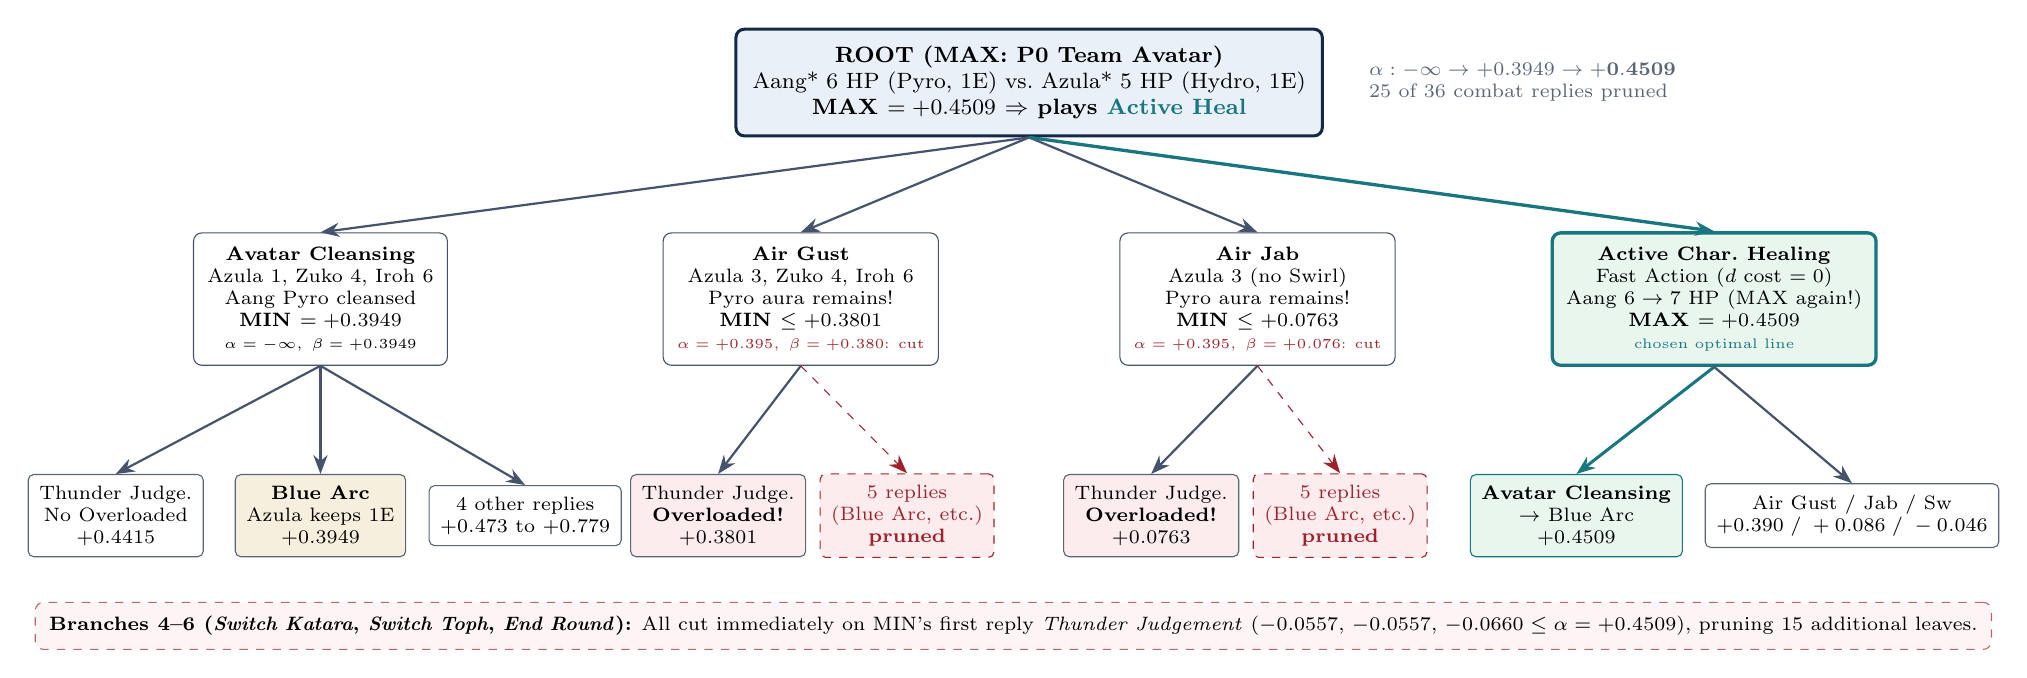
\begin{tikzpicture}[
  rootbox/.style={rectangle, rounded corners=3pt, draw=navy, line width=1.1pt, fill=softblue, inner sep=6pt, align=center, font=\footnotesize},
  midbox/.style={rectangle, rounded corners=3pt, draw=navy!80, fill=white, inner sep=5pt, align=center, font=\scriptsize, minimum width=3.2cm},
  winbox/.style={rectangle, rounded corners=3pt, draw=tealaccent, line width=1.2pt, fill=softgreen, inner sep=5pt, align=center, font=\scriptsize, minimum width=3.4cm},
  leaf/.style={rectangle, rounded corners=2pt, draw=slate, fill=white, inner sep=4pt, align=center, font=\scriptsize, minimum width=2.05cm},
  pruned/.style={rectangle, rounded corners=2pt, dashed, draw=crimson, fill=softred, inner sep=4pt, align=center, font=\scriptsize, text=crimson, minimum width=2.05cm},
  arr/.style={-{Stealth[length=2.4mm]}, thick, color=navy!80},
  parr/.style={-{Stealth[length=2.4mm]}, dashed, color=crimson}
]
  % Root
  \node[rootbox] (R) at (0,0) {\textbf{ROOT (MAX: P0 Team Avatar)}\\Aang* 6~HP (Pyro, 1E) vs.\ Azula* 5~HP (Hydro, 1E)\\\textbf{MAX $= +0.4509$ $\Rightarrow$ plays \textcolor{tealaccent}{Active Heal}}};
  \node[right=0.45cm of R, font=\scriptsize, color=slate, align=left] {$\alpha: -\infty \to +0.3949 \to \mathbf{+0.4509}$\\25 of 36 combat replies pruned};

  % Level 1 (well-spaced across [-9.2, +8.8])
  \node[midbox] (B0) at (-9.0,-2.75) {\textbf{Avatar Cleansing}\\Azula 1, Zuko 4, Iroh 6\\Aang Pyro cleansed\\\textbf{MIN $= +0.3949$}\\{\tiny $\alpha=-\infty,\;\beta=+0.3949$}};
  \node[midbox] (B1) at (-2.9,-2.75) {\textbf{Air Gust}\\Azula 3, Zuko 4, Iroh 6\\Pyro aura remains!\\\textbf{MIN $\le +0.3801$}\\{\tiny\color{crimson} $\alpha=+0.395,\;\beta=+0.380$: cut}};
  \node[midbox] (B2) at (2.9,-2.75) {\textbf{Air Jab}\\Azula 3 (no Swirl)\\Pyro aura remains!\\\textbf{MIN $\le +0.0763$}\\{\tiny\color{crimson} $\alpha=+0.395,\;\beta=+0.076$: cut}};
  \node[winbox] (B3) at (8.7,-2.75) {\textbf{Active Char.\ Healing}\\Fast Action ($d$ cost $= 0$)\\Aang $6 \to 7$~HP (MAX again!)\\\textbf{MAX $= +0.4509$}\\{\tiny\color{tealaccent} chosen optimal line}};

  \draw[arr] (R.south) -- (B0.north);
  \draw[arr] (R.south) -- (B1.north);
  \draw[arr] (R.south) -- (B2.north);
  \draw[arr, color=tealaccent, line width=1.2pt] (R.south) -- (B3.north);

  % Level 2 under B0 (clean generous gaps!)
  \node[leaf] (L00) at (-11.6,-5.5) {Thunder Judge.\\No Overloaded\\$+0.4415$};
  \node[leaf, fill=goldlight] (L01) at (-9.0,-5.5) {\textbf{Blue Arc}\\Azula keeps 1E\\\textbf{$+0.3949$}};
  \node[leaf] (L02) at (-6.4,-5.5) {4 other replies\\$+0.473$ to $+0.779$};
  \draw[arr] (B0.south) -- (L00.north);
  \draw[arr] (B0.south) -- (L01.north);
  \draw[arr] (B0.south) -- (L02.north);

  % Level 2 under B1
  \node[leaf, fill=softred] (L10) at (-3.95,-5.5) {Thunder Judge.\\\textbf{Overloaded!}\\$+0.3801$};
  \node[pruned] (L11) at (-1.55,-5.5) {5 replies\\(Blue Arc, etc.)\\\textbf{pruned}};
  \draw[arr] (B1.south) -- (L10.north);
  \draw[parr] (B1.south) -- (L11.north);

  % Level 2 under B2
  \node[leaf, fill=softred] (L20) at (1.55,-5.5) {Thunder Judge.\\\textbf{Overloaded!}\\$+0.0763$};
  \node[pruned] (L21) at (3.95,-5.5) {5 replies\\(Blue Arc, etc.)\\\textbf{pruned}};
  \draw[arr] (B2.south) -- (L20.north);
  \draw[parr] (B2.south) -- (L21.north);

  % Level 2 under B3 (Fast action follow-ups, crisp separation)
  \node[leaf, draw=tealaccent, fill=softgreen] (L30) at (6.95,-5.5) {\textbf{Avatar Cleansing}\\$\to$ Blue Arc\\\textbf{$+0.4509$}};
  \node[leaf] (L31) at (10.45,-5.5) {Air Gust / Jab / Sw\\$+0.390 \;/\; +0.086 \;/\; -0.046$};
  \draw[arr, color=tealaccent, line width=1.1pt] (B3.south) -- (L30.north);
  \draw[arr] (B3.south) -- (L31.north);

  % Note for branches 4-6
  \node[rectangle, rounded corners=3pt, draw=crimson!70, dashed, fill=softred!60, font=\scriptsize, inner sep=5pt, align=center] at (-0.2,-6.9)
    {\textbf{Branches 4--6 (\emph{Switch Katara}, \emph{Switch Toph}, \emph{End Round}):} All cut immediately on MIN's first reply \emph{Thunder Judgement} ($-0.0557$, $-0.0557$, $-0.0660 \le \alpha = +0.4509$), pruning 15 additional leaves.};
\end{tikzpicture}}
\caption{Engine-verified depth-2 Alpha-Beta search tree for the Round~2 Avatar position. Zero-cost Fast Action depth preservation uncovers \emph{Active Character Healing} $\to$ \emph{Avatar Cleansing} ($+0.4509$), while move ordering prunes 25 of 36 combat replies.}
\label{fig:ab-tree}
\end{figure}

At full \emph{Normal} depth~4, \texttt{TCGSearcher.best\_move} explores only 500 nodes and still selects \textbf{Active Character Healing} (depth-4 score $+0.4291$).

\subsection{IS-MCTS, Step by Step}

On the exact same state, \emph{Hard} first scores all 7 moves via depth-4 Alpha-Beta to form the Top-4 Shortlist \{\emph{Air Gust}, \emph{Active Character Healing}, \emph{Avatar Cleansing}, \emph{Switch $\to$ Toph}\}, then runs $N = 700$ determinized IS-MCTS iterations ($\ln(701) = 6.5525$, $C = 0.9$). At termination, the UCT scores (Equation~\ref{eq:uct}) of the top two contenders are tightly balanced:
\[
  \text{Air Gust}: \frac{134.31}{224} + 0.9\sqrt{\frac{6.5525}{225}} = 0.7532, \qquad
  \text{Avatar Cleansing}: \frac{129.54}{217} + 0.9\sqrt{\frac{6.5525}{218}} = 0.7530.
\]
\emph{Hard} returns the most-visited child: \textbf{Air Gust} ($n = 224$), narrowly ahead of \emph{Avatar Cleansing} ($n = 217$). Figure~\ref{fig:mcts-tree} illustrates the resulting search tree. Notably, compared to \emph{Pure IS-MCTS} without the Top-4 shortlist (where the leader received only $n=143$ visits across 7 moves), our Alpha-Beta shortlist increased visit concentration on the leading moves by \textbf{+56.6\%}.

\begin{figure}[H]
\centering
\resizebox{\textwidth}{!}{%
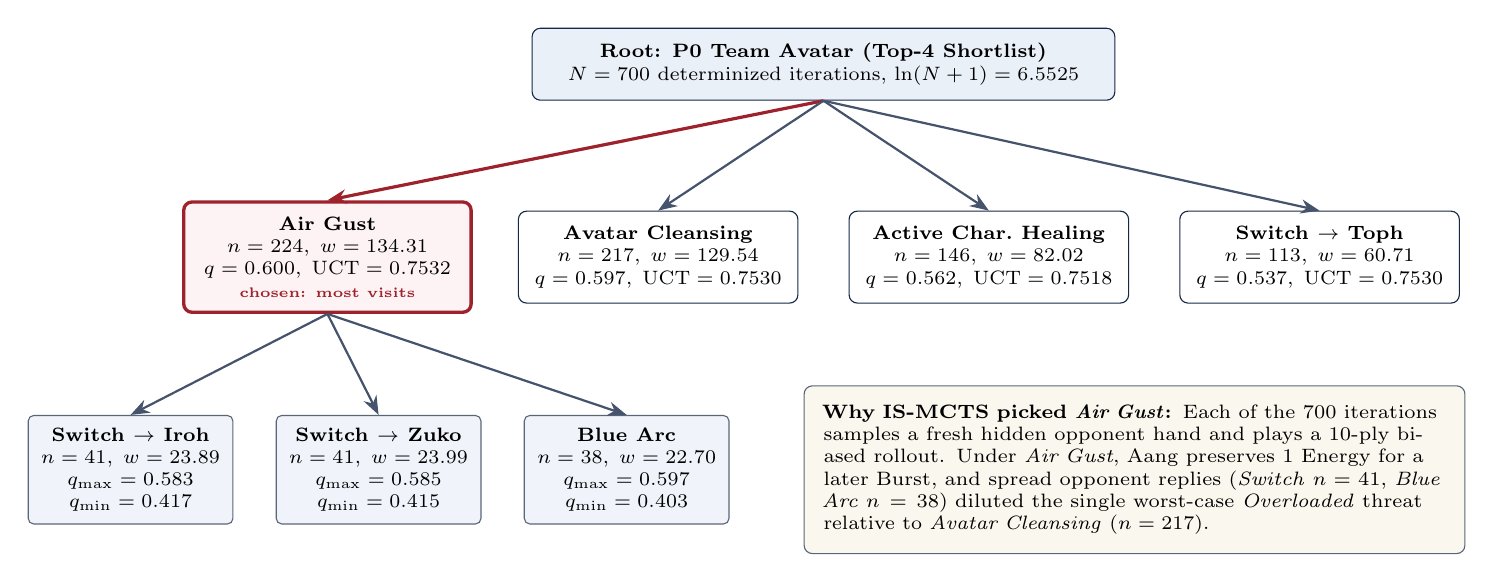
\begin{tikzpicture}[
  nodebox/.style={rectangle, rounded corners=3pt, draw=navy, fill=white, inner sep=5.5pt, align=center, font=\scriptsize, minimum width=3.55cm},
  best/.style={rectangle, rounded corners=3pt, draw=crimson, line width=1.2pt, fill=softred!65, inner sep=5.5pt, align=center, font=\scriptsize, minimum width=3.65cm},
  sub/.style={rectangle, rounded corners=2pt, draw=slate, fill=softblue!70, inner sep=4.5pt, align=center, font=\scriptsize, minimum width=2.85cm},
  arr/.style={-{Stealth[length=2.4mm]}, thick, color=navy!80}
]
  \node[nodebox, fill=softblue, minimum width=7.4cm] (R) at (0,0) {\textbf{Root: P0 Team Avatar (Top-4 Shortlist)}\\$N = 700$ determinized iterations, $\ln(N+1) = 6.5525$};

  % Four well-spaced root children (x = -6.3, -2.1, +2.1, +6.3 -> 0.6cm gaps!)
  \node[best]    (C1) at (-6.3,-2.45) {\textbf{Air Gust}\\$n = 224,\; w = 134.31$\\$q = 0.600,\; \mathrm{UCT} = 0.7532$\\{\tiny\bfseries\color{crimson} chosen: most visits}};
  \node[nodebox] (C2) at (-2.1,-2.45) {\textbf{Avatar Cleansing}\\$n = 217,\; w = 129.54$\\$q = 0.597,\; \mathrm{UCT} = 0.7530$};
  \node[nodebox] (C3) at (2.1,-2.45)  {\textbf{Active Char.\ Healing}\\$n = 146,\; w = 82.02$\\$q = 0.562,\; \mathrm{UCT} = 0.7518$};
  \node[nodebox] (C4) at (6.3,-2.45)  {\textbf{Switch $\to$ Toph}\\$n = 113,\; w = 60.71$\\$q = 0.537,\; \mathrm{UCT} = 0.7530$};

  \draw[arr, color=crimson, line width=1.15pt] (R.south) -- (C1.north);
  \draw[arr] (R.south) -- (C2.north);
  \draw[arr] (R.south) -- (C3.north);
  \draw[arr] (R.south) -- (C4.north);

  % Three well-spaced opponent replies under Air Gust (compact 2-line q_max/q_min, zero overlap!)
  \node[sub, minimum width=2.6cm] (S1) at (-8.8,-5.15) {\textbf{Switch $\to$ Iroh}\\$n = 41,\; w = 23.89$\\$q_{\text{max}}=0.583$\\$q_{\text{min}}=0.417$};
  \node[sub, minimum width=2.6cm] (S2) at (-5.65,-5.15) {\textbf{Switch $\to$ Zuko}\\$n = 41,\; w = 23.99$\\$q_{\text{max}}=0.585$\\$q_{\text{min}}=0.415$};
  \node[sub, minimum width=2.6cm] (S3) at (-2.5,-5.15) {\textbf{Blue Arc}\\$n = 38,\; w = 22.70$\\$q_{\text{max}}=0.597$\\$q_{\text{min}}=0.403$};

  \draw[arr] (C1.south) -- (S1.north);
  \draw[arr] (C1.south) -- (S2.north);
  \draw[arr] (C1.south) -- (S3.north);

  % Explanation callout box cleanly to the right
  \node[rectangle, rounded corners=3pt, draw=slate, fill=goldlight!50, text width=7.9cm, inner sep=7pt, font=\scriptsize, align=left] at (3.95,-5.15)
    {\textbf{Why IS-MCTS picked \emph{Air Gust}:} Each of the 700 iterations samples a fresh hidden opponent hand and plays a 10-ply biased rollout. Under \emph{Air Gust}, Aang preserves 1~Energy for a later Burst, and spread opponent replies (\emph{Switch} $n=41$, \emph{Blue Arc} $n=38$) diluted the single worst-case \emph{Overloaded} threat relative to \emph{Avatar Cleansing} ($n=217$).};
\end{tikzpicture}}
\caption{Engine-verified IS-MCTS search tree ($N=700$ iterations, Top-4 Alpha-Beta shortlist) on the same Round~2 position.}
\label{fig:mcts-tree}
\end{figure}

\subsection{CSP Smart Dice Payment Trace}

Before returning the chosen action, \texttt{TCGDicePay.smart\_pay} optimizes which dice indices are spent. Suppose Team Avatar (\texttt{keep = \{Anemo, Hydro, Geo\}}) casts \emph{Air Gust} (2~Anemo + 1~Any) from dice \texttt{[0:Pyro, 1:Anemo, 2:Geo, 3:Anemo, 4:Omni, 5:Hydro]}:
\begin{itemize}[leftmargin=1.4em, itemsep=1pt]
  \item Variables $e_0, e_1$ have domain $\{1, 3, 4\}$ (Anemo or Omni); $u_0$ has domain $\{0,1,2,3,4,5\}$ under \texttt{AllDiff}.
  \item Value weights rank \texttt{0:Pyro} ($1.0$), \texttt{1,3:Anemo} ($3/2 = 1.5$), \texttt{2:Geo, 5:Hydro} ($3.0$), and \texttt{4:Omni} ($100.0$).
  \item MRV assigns tight slots $e_0 \gets 1$ and $e_1 \gets 3$; forward checking removes $\{1,3\}$ from $u_0$, which selects off-element \texttt{0:Pyro} $\Rightarrow$ output \textbf{\texttt{[0, 1, 3]}}, preserving \texttt{Omni}, \texttt{Geo}, and \texttt{Hydro}.
\end{itemize}
Similarly, paying 2~Same-Type for \emph{Aang's Glider Staff} from \texttt{[Pyro, Pyro, Anemo, Anemo, Omni, Hydro]} chooses the off-element Pyro pair \textbf{\texttt{[0, 1]}}, leaving both Anemo dice and Omni intact for \emph{Avatar Cleansing}.

\subsection{Comparing Normal (Alpha-Beta) and Hard (Hybrid IS-MCTS)}

In this exact position, \emph{Normal} (Alpha-Beta) chose \textbf{Active Character Healing} (planning \emph{Avatar Cleansing} next to cleanse Pyro and dodge Overloaded), whereas \emph{Hard} (IS-MCTS) chose \textbf{Air Gust} ($n=224$ vs.\ $217$). Alpha-Beta systematically checks \emph{every} worst-case reply at depth 2--4 and preserves depth on Fast Actions, immediately spotting the exact Overloaded punishment. IS-MCTS excels at evaluating multi-round trajectories across hidden hands, but with 700 stochastic rollouts split over several opponent replies, a razor-thin 1-move tactical trap can be partially masked by rollout noise.

% ==============================================================================
% SECTION 9: RESULTS
% ==============================================================================
\section{Results: Multi-Tier AI Benchmark}

To evaluate playing strength and runtime fairly, we ran a \textbf{12-game headless AI-vs-AI tournament} inside Godot~4 across all three preset decks (\emph{Team Avatar}, \emph{Fire Nation Royals}, \emph{Lotus \& Rebels}), alternating first player and team assignments across every pairing (Table~\ref{tab:tournament}). Table~\ref{tab:totals} aggregates win rates, average surviving HP, and average Action-Phase thinking time per move.

\begin{table}[H]
\centering
\caption{Twelve full AI-vs-AI matches across Easy, Normal, and Hard tiers (alternating first player and preset decks).}
\label{tab:tournament}
\footnotesize
\setlength{\tabcolsep}{4.5pt}
\begin{tabular}{@{}cllccclrr@{}}
\toprule
 & \multicolumn{2}{c}{Matchup (First vs.\ Second)} & & & & & \multicolumn{2}{c}{Avg.\ Time / Move} \\
\cmidrule(lr){2-3} \cmidrule(lr){8-9}
Game & Player 0 (First) & Player 1 (Second) & Rds & Final HP & Winner & & P0 & P1 \\
\midrule
1 & Normal (\emph{Team Avatar}) & Easy (\emph{Fire Royals}) & 5 & 16--0 & \textbf{Normal} & & 177.6~ms & 1.5~ms \\
2 & Easy (\emph{Fire Royals}) & Normal (\emph{Team Avatar}) & 7 & 0--4 & \textbf{Normal} & & 1.7~ms & 207.8~ms \\
3 & Normal (\emph{Lotus \& Reb.}) & Easy (\emph{Team Avatar}) & 5 & 11--0 & \textbf{Normal} & & 271.0~ms & 1.7~ms \\
4 & Easy (\emph{Team Avatar}) & Normal (\emph{Lotus \& Reb.}) & 5 & 0--15 & \textbf{Normal} & & 1.5~ms & 290.5~ms \\
\midrule
5 & Hard (\emph{Team Avatar}) & Easy (\emph{Fire Royals}) & 6 & 9--0 & \textbf{Hard} & & 839.1~ms & 1.6~ms \\
6 & Easy (\emph{Fire Royals}) & Hard (\emph{Team Avatar}) & 5 & 0--21 & \textbf{Hard} & & 1.7~ms & 635.9~ms \\
\midrule
7 & Hard (\emph{Team Avatar}) & Normal (\emph{Fire Royals}) & 7 & 0--7 & \textbf{Normal} & & 637.5~ms & 183.5~ms \\
8 & Normal (\emph{Fire Royals}) & Hard (\emph{Team Avatar}) & 5 & 7--0 & \textbf{Normal} & & 244.0~ms & 502.2~ms \\
9 & Hard (\emph{Lotus \& Reb.}) & Normal (\emph{Team Avatar}) & 6 & 12--0 & \textbf{Hard} & & 851.3~ms & 126.8~ms \\
10 & Normal (\emph{Team Avatar}) & Hard (\emph{Lotus \& Reb.}) & 6 & 0--4 & \textbf{Hard} & & 276.5~ms & 687.7~ms \\
11 & Hard (\emph{Fire Royals}) & Normal (\emph{Lotus \& Reb.}) & 5 & 0--11 & \textbf{Normal} & & 652.5~ms & 166.6~ms \\
12 & Normal (\emph{Lotus \& Reb.}) & Hard (\emph{Fire Royals}) & 5 & 7--0 & \textbf{Normal} & & 194.5~ms & 610.7~ms \\
\bottomrule
\end{tabular}
\end{table}

\begin{table}[H]
\centering
\caption{Aggregate tournament performance across all 12 games.}
\label{tab:totals}
\small
\begin{tabular}{@{}lcccc@{}}
\toprule
AI Tier & Games Won & Win Rate & Avg.\ Remaining HP & Avg.\ Time / Action Move \\
\midrule
\textbf{Easy} (Fuzzy 1-ply) & 0 / 6 & 0.0\% & 0.0 & 1.6~ms (105 moves) \\
\textbf{Normal} (A* + Alpha-Beta) & 8 / 10 & \textbf{80.0\%} & \textbf{7.8} & 212.1~ms (296 moves) \\
\textbf{Hard} (A* + AB + IS-MCTS) & 4 / 8 & 50.0\% & 5.8 & 675.1~ms (238 moves) \\
\bottomrule
\end{tabular}
\end{table}

Two clear empirical conclusions emerge:
\begin{enumerate}[leftmargin=1.4em, itemsep=2pt]
  \item \textbf{Search + Lethal Planning Dominate Greedy Play:} Both \emph{Normal} (4--0) and \emph{Hard} (2--0) swept \emph{Easy} 6--0 regardless of turn order or deck, confirming the massive value of A* lethal combos, multi-ply reaction awareness, and zero-cost fast-action look-ahead.
  \item \textbf{Alpha-Beta Edges Out Shortlisted IS-MCTS Head-to-Head:} Against \emph{Hard}, \emph{Normal} won 4--2 while running more than \textbf{3$\times$ faster} (212.1~ms vs.\ 675.1~ms per move). Just as observed in our Section~\ref{sec:tree} decision tree trace, Resonance's sharp 1-turn elemental reaction punishments (Overloaded $+2$ + forced switch, Aang $+2$ Swirl, Stunned) reward Alpha-Beta's exact worst-case reply verification over noisy finite-budget rollouts.
\end{enumerate}

\subsection{When Hard (IS-MCTS) Won}

\noindent
\begin{minipage}[t]{0.46\textwidth}
\vspace{0pt}
Despite Alpha-Beta's tactical edge in sharp Fire-vs-Fire exchanges, \emph{Hard} swept both \emph{Lotus \& Rebels} vs.\ \emph{Team Avatar} matchups (Games~9 and~10, winning 12--0 going first and 4--0 going second). In slower 6-round attrition games featuring Toph's shields and Katara's healing, IS-MCTS's 10-ply biased rollouts and multi-world determinization captured long-horizon sustain value beyond Alpha-Beta's 4-ply horizon. Figure~\ref{fig:victory-shot} shows a clean match victory screen upon knocking out all three opposing characters.
\end{minipage}\hfill
\begin{minipage}[t]{0.50\textwidth}
\vspace{0pt}
\centering
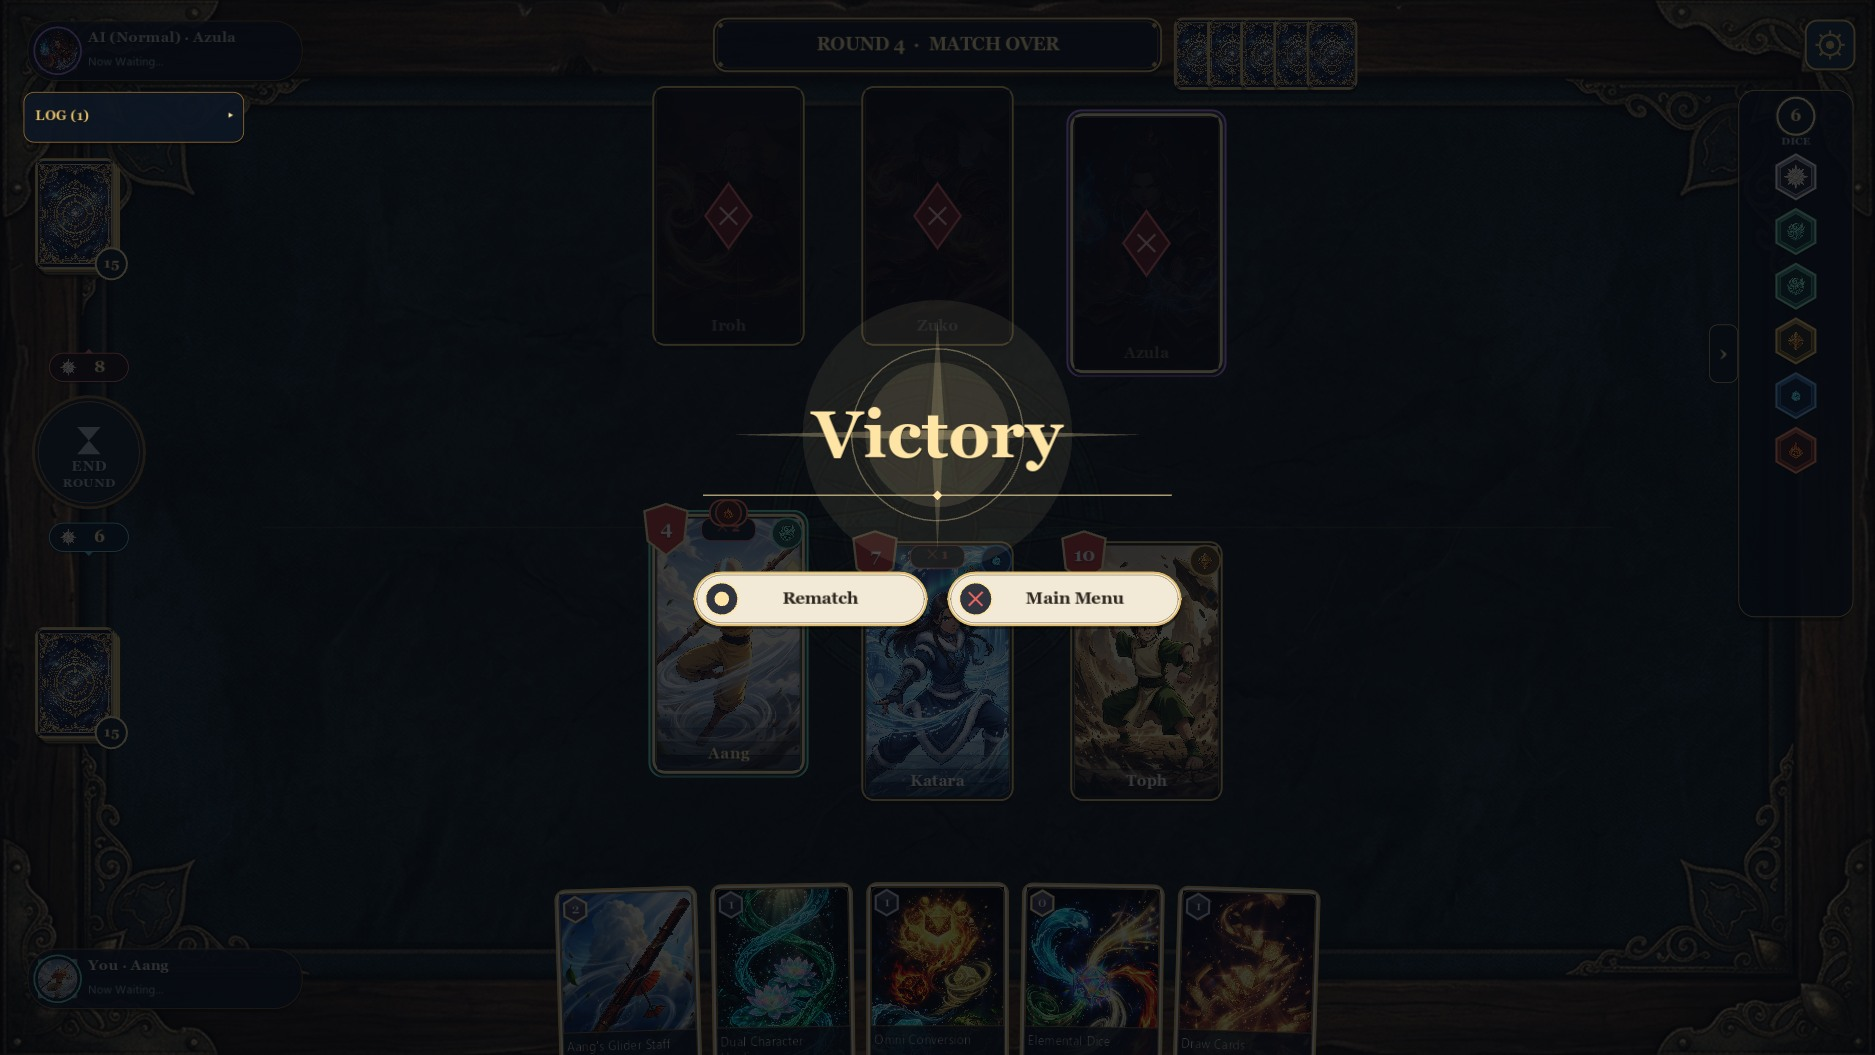
\includegraphics[width=\textwidth]{images/ui_victory_clean.jpg}
\captionof{figure}{Clean match victory overlay after defeating all three opposing characters.}
\label{fig:victory-shot}
\end{minipage}

% ==============================================================================
% SECTION 10: CHALLENGES AND SOLUTIONS
% ==============================================================================
\section{Challenges and Solutions}

Table~\ref{tab:challenges} records the main algorithmic and engineering issues encountered during development and how each was resolved.

\begin{table}[H]
\centering
\caption{Key engineering and AI challenges encountered and their verified solutions.}
\label{tab:challenges}
\small
\begin{tabularx}{\textwidth}{@{}L{5.6cm} Y@{}}
\toprule
Challenge & How We Solved It \\
\midrule
Fast-action horizon distortion in Minimax & Assigned $\fn{Cost}(a)=0$ to Fast Actions and $1$ to Combat Actions, ensuring opponent replies stay inside the search horizon. \\
Imperfect-information leakage & Built \texttt{TCGWorld.determinize} to sample legal opponent hands and shuffle decks before every search; verified zero cheating in automated AI tests. \\
MCTS visit dilution across weak moves & Added an Alpha-Beta Top-4 root shortlist on Hard, boosting visit concentration on the best candidates by $+56.6\%$. \\
Same-Type dice costs (e.g.\ 2~Same weapons) & Extended \texttt{TCGDicePay} to rank candidate element pairs by off-element preference before invoking the \texttt{AllDiff} MRV CSP solver. \\
Azula Burst + Overloaded stunned wrong target & Added \texttt{last\_damage\_target} tracking in \texttt{TCGEffectContext} so \emph{Stunned} attaches to the struck character even after Overloaded forces a switch. \\
Mulligan \& \emph{Swap Cards} clicks swallowed by drag & Disabled card dragging during swap selection and changed deck replenishment to draw replacements \emph{before} shuffling returned cards back. \\
Payment Cancel (\texttt{X}) overlapped Settings button & Repositioned \texttt{\_pay\_cancel\_rect()} cleanly beside the Settings gear and validated layout across 16:9, 19.5:9, and 4:3 viewports. \\
\bottomrule
\end{tabularx}
\end{table}

% ==============================================================================
% SECTION 11: LIMITATIONS AND FUTURE WORK
% ==============================================================================
\section{Limitations and Future Work}

\noindent
\begin{minipage}[t]{0.475\textwidth}
\textbf{Limitations}
\begin{itemize}[leftmargin=1.2em, itemsep=1pt, topsep=2pt]
  \item Fuzzy rule outputs and evaluation weights were tuned by hand rather than learned from self-play.
  \item Aura vulnerability in \texttt{TCGEvaluate} checks core aura-to-aura reactions (\emph{Vaporize}, \emph{Overloaded}, \emph{Electro-Charged}), omitting \emph{Swirl} and \emph{Crystallize} threat penalties.
  \item IS-MCTS samples opponent hands uniformly from legal deck cards rather than updating a Bayesian belief from played cards.
  \item The benchmark evaluated 12 full games over the 3 preset decks; larger statistical sweeps would tighten confidence intervals.
  \item Currently supports local single-device play (vs.\ AI, hotseat PvP, AI vs.\ AI) with a 6-character roster.
\end{itemize}
\end{minipage}\hfill
\begin{minipage}[t]{0.475\textwidth}
\textbf{Future Work}
\begin{itemize}[leftmargin=1.2em, itemsep=1pt, topsep=2pt]
  \item Optimize evaluation and Fuzzy parameters automatically via evolutionary self-play or temporal-difference learning.
  \item Add Zobrist hashing and a transposition table to Alpha-Beta to reach depth 5--6 within the same 0.6~s budget.
  \item Upgrade IS-MCTS determinization to track observed opponent cards and narrow the legal hand-sampling pool.
  \item Include Anemo \emph{Swirl} and Geo \emph{Crystallize} reaction threats directly inside \texttt{TCGEvaluate}.
  \item Expand the roster (introducing Cryo characters to unlock \emph{Melt} and \emph{Frozen}) and add networked LAN/online multiplayer.
\end{itemize}
\end{minipage}

% ==============================================================================
% SECTION 12: CONCLUSION
% ==============================================================================
\section{Conclusion}

We designed, implemented, and verified \textbf{Resonance: Genius Invokation TCG (Avatar Edition)}, a complete tactical card game in Godot~4 backed by a deterministic data-driven rules engine, 116 passing automated tests, and a six-component AI architecture. By integrating Sugeno Fuzzy Logic, informed A* Lethal Planning, Iterative-Deepening Alpha-Beta with zero-cost Fast Action depth tracking, Shortlisted Determinized IS-MCTS, and MRV Forward-Checking CSP solvers, our AI agents handle hidden hands, stochastic dice, and multi-action turns without freezing the interface or peeking at hidden state. Both our step-by-step decision tree analysis and our 12-game tournament demonstrate that search and lethal planning decisively beat greedy play (6--0 vs.\ Easy), while Iterative-Deepening Alpha-Beta achieves the strongest overall balance of tactical accuracy (80\% win rate) and responsiveness (212~ms/move), complemented by IS-MCTS's strength in longer multi-round attrition matches.

% ==============================================================================
% REFERENCES
% ==============================================================================
\begin{thebibliography}{9}
\footnotesize
\setlength{\itemsep}{1pt}
\setlength{\parskip}{0pt}
\bibitem{russell}
S.~Russell and P.~Norvig, \emph{Artificial Intelligence: A Modern Approach}, 4th~ed.\ Pearson, 2021.

\bibitem{knuth}
D.~E.~Knuth and R.~W.~Moore, ``An analysis of alpha-beta pruning,'' \emph{Artificial Intelligence}, vol.~6, no.~4, pp.~293--326, 1975.

\bibitem{hart}
P.~E.~Hart, N.~J.~Nilsson, and B.~Raphael, ``A formal basis for the heuristic determination of minimum cost paths,'' \emph{IEEE Trans.\ Systems Science and Cybernetics}, vol.~4, no.~2, pp.~100--107, 1968.

\bibitem{takagi}
T.~Takagi and M.~Sugeno, ``Fuzzy identification of systems and its applications to modeling and control,'' \emph{IEEE Trans.\ Systems, Man, and Cybernetics}, vol.~SMC-15, no.~1, pp.~116--132, 1985.

\bibitem{kocsis}
L.~Kocsis and C.~Szepesv\'{a}ri, ``Bandit based Monte-Carlo planning,'' in \emph{Proc.\ ECML}, 2006, pp.~282--293.

\bibitem{browne}
C.~B.~Browne et al., ``A survey of Monte Carlo tree search methods,'' \emph{IEEE Trans.\ Computational Intelligence and AI in Games}, vol.~4, no.~1, pp.~1--43, 2012.

\bibitem{cowling}
P.~I.~Cowling, E.~J.~Powley, and D.~Whitehouse, ``Information Set Monte Carlo Tree Search,'' \emph{IEEE Trans.\ Computational Intelligence and AI in Games}, vol.~4, no.~2, pp.~120--143, 2012.
\end{thebibliography}

\end{document}
